\documentclass[11pt,a4paper,titlepage]{article}
\usepackage[utf8]{inputenc}
\usepackage[german]{babel}
\usepackage[T1]{fontenc}
\usepackage{amsmath}
\usepackage{amsfonts}
\usepackage{amssymb}
\usepackage{graphicx}
\usepackage{xcolor}
\usepackage{wrapfig}
\usepackage{caption}
\usepackage{subcaption}
\setlength{\parindent}{0px}
\definecolor{htw}{RGB}{125, 173, 24}

\usepackage{times}
\usepackage{float} 
\usepackage{calc}
\usepackage{helvet}
\usepackage[singlespacing]{setspace}
\usepackage[bottom]{footmisc} % footnote at the bottom of the page
\PassOptionsToPackage{hyphens}{url}
\usepackage{hyperref}
\usepackage{footnotebackref}

\usepackage[margin=1in]{geometry}

\usepackage[figurename=Abb.,tablename=Tab.]{caption}
\usepackage[ngerman, nameinlink]{cleveref}
\usepackage{tabularx}
\usepackage{listings}
\usepackage{fancyvrb}

\usepackage[indent=0pt]{parskip}

\usepackage[inkscapeformat=png]{svg}

\crefname{table}{Tab.}{Tab.}
\Crefname{table}{Tab.}{Tab.}
\crefname{lstlisting}{Code-Ausschnitt}{Code-Ausschnitt}

% Boxen um Links entfernen
\hypersetup{
  colorlinks,
  linkcolor={blue!70!black}
}

\usepackage{color}

\definecolor{dkgreen}{rgb}{0,0.6,0}
\definecolor{gray}{rgb}{0.5,0.5,0.5}
\definecolor{mauve}{rgb}{0.58,0,0.82}

\lstdefinestyle{customc}{
  numbers=left,
  belowcaptionskip=1\baselineskip,
  breaklines=true,
  frame=L,
  xleftmargin=25pt,
  language=C,
  showstringspaces=false,
  basicstyle=\footnotesize\ttfamily,
  keywordstyle=\bfseries\color{green!40!black},
  commentstyle=\itshape\color{purple!40!black},
  identifierstyle=\color{blue},
  stringstyle=\color{orange},
}

\lstset{frame=tb,
  language=C,
  aboveskip=3mm,
  belowskip=3mm,
  showstringspaces=false,
  columns=flexible,
  basicstyle={\small\ttfamily},
  numbers=none,
  numberstyle=\tiny\color{gray},
  keywordstyle=\color{blue},
  commentstyle=\color{dkgreen},
  stringstyle=\color{mauve},
  breaklines=true,
  breakatwhitespace=true,
  tabsize=3,
  numbers=left
}

% Namen von Listings verändern
\renewcommand{\lstlistingname}{Code-Ausschnitt}
\renewcommand{\lstlistlistingname}{Liste von Code-Ausschnitten}

\begin{document}

\begin{titlepage}
    \centering




    \begin{figure}
        \centering
        
\includegraphics[scale=1]{htw-berlin_logo.jpg}
    \end{figure}



    {\LARGE\bfseries CE31 Embedded Systems}


    \vspace{2cm}

    {\Large Laborprojekt I²C-Kommunikation}

    Gruppe 6

    \vspace{1cm}

    {\large Kevin Hübner | 570746}\\
    {\large Tobit Zander | 582020}

    \vspace{0.1cm}





\end{titlepage}

\newpage
\tableofcontents
\listoffigures
\listoftables
\lstlistoflistings
\newpage

\section{Projekt Idee}
In diesem Labor werden zwei Nucleo-Boards miteinander verbunden,
um Daten über das I²C-Protokoll (oder auch I2C) auszutauschen.\\
Ein Board fungiert dabei als Master und das andere Board als Slave.\\

Das Master-Board ist mit einem Temperatur- und Luftfeuchtigkeitssensor (AM2302) ausgestattet.
Dabei misst dieses Board in einem 5 Sekundentakt die aktuellen Werte
\footnote{In einem Datensatz liegen sowohl die Luftfeuchtigkeits- als auch die Temperaturwert. Es gibt keine Möglichkeit die Werte einzeln zuerfragen.}
und sendet abwechselnd Luftfeuchtigkeit und Temperatur über die I²C-Schnittstelle zum Slave.\\

Das andere Nucleo-Board ist mit einem Modul ausgestattet, das aus vier sieben-Segment-Anzeigen (TM1637) besteht.
Diese Anzeigen dienen der Darstellung der empfangenen Daten.
Das Board stellt dabei entweder Luftfeuchtigkeit oder Temperatur dar,
jenachdem welchen Wert es über das I2C-Protokoll vom ersten Board erhält.\\

In diesem Labor wird Schritt für Schritt durch den Entwicklungsprozess geführt und dabei aufgetretene Probleme näher erläutert.

\section{Bauteilliste}
Folgende Bauteile kamen für dieses Projekt zum Einsatz:\\

Auf Seiten der Darstellung:
\begin{itemize}
    \item Nucleo-F042K6
    \item TM1637
          \footnote{TM1637 Datenblatt: \url{https://cdn.shopify.com/s/files/1/1509/1638/files/4-Bit_7-Segment_LED_Display_Datenblatt_AZ-Delivery_Vertriebs_GmbH.pdf}}
          (4-stellige 7-Segment-Anzeige)
\end{itemize}

Auf Seiten der Datenerhebung:
\begin{itemize}
    \item Nucleo-L432KC
    \item AM2302
          \footnote{AM2302 Datenblatt: \url{https://files.seeedstudio.com/wiki/Grove-Temperature_and_Humidity_Sensor_Pro/res/AM2302-EN.pdf}}
          (Temperatur- und Luftfeuchtigkeitssensor)
\end{itemize}

Zum Verbindungsaufbau zwischen den beiden Mikrocontrollern:
\begin{itemize}
    \item 2x 2k Ohm (als PullUp-Widerstände)
\end{itemize}

Weiterhin wurden während des Entwicklungsprozesses zusätzliche Hilfsmittel eingesetzt:
\begin{itemize}
    \item Logic Analyzer
    \item Arduino (hier ein NANO EVERY)
    \item Handyprobe HP3 (digital Osziloskop)
\end{itemize}

\newpage
\section{Umsetzung}
Im folgenden wird nun die Umsetzung des Projektes detailiert beschrieben.

Das gesammte Projekt liegt dabei versionsverwaltet auf dem HTW eingenen GitLab-Server unter
\url{https://gitlab.rz.htw-berlin.de/s0582020/ce31-embd-gruppe-6-tz-kh}.
Dort sind auch, unter der README-Datei im Root-Verzeichnis,
\footnote{\url{https://gitlab.rz.htw-berlin.de/s0582020/ce31-embd-gruppe-6-tz-kh/-/blob/main/README.md}}
alle Informationen zum Bauen der Projekte erhältlich.

\subsection{Temperatur- und Luftfeuchtigkeitssensor (Tobit Zander)}

\subsubsection{Sensor verstehen}
Bevor mit der Implementierung begonnen werden konnte, wurde zunächst das Datenblatt
\footnote{\url{https://files.seeedstudio.com/wiki/Grove-Temperature_and_Humidity_Sensor_Pro/res/AM2302-EN.pdf}}
des Luftfeuchtigkeits- und Temperartursensor (AM2302) herausgesucht und evaluiert.\\

Der für dieses Projekt genutzte Sensor nutzt ein \textit{ONE-WIRE} Protokoll zur Übertragung der Daten.\\
Dieses Protokoll sieht dabei ledigleich nur eine Datenverbindung vor.
Um allerdings dennoch eine \textit{bidirecktionale} Verdingung zwischen Mikrocontroller und Sensor bereitstellen zu können,
kommt das sog. \textit{wired AND} zum Einsatz.

Das heißt, alle Teilnehmner schalten die Datenpins \textit{hochohmig}.
Ein benötigter \textit{Pull up-Widerstand} zieht dann den Pegel automatisch auf \textit{High},
solange alle Beteiligten ihre Pins hochohmig gestellt haben.\\

Sobald eine Null (entspricht dem \textit{Low}-Pegel) von einem der beiden (Mikrocontroller oder der Sensor) übertragen werden soll,
kann die Busleitung aktiv auf \textit{Low} gezogen werden.
Eine Eins entsteht wieder von selbst,
wenn derjenige den Datenpin auf hochohmig stellt und die PullUp-Widerstände die Leitung auf High ziehen.

Dieses Prinzip wird auch vom I²C Bus genutzt.
Und deshalt die beiden 2k Ohm Widerstände aus der Bauteilliste.\\

Das Senden der Messwerte durch den Sensor wird durch das Senden eines \textit{Startsignal} getriggert (siehe $T_{be}$ in \cref{fig:ONE-WIRE}).
Nach Freigabe des Busses ($T_{go}$) durch den Mikrocontroller folgt eine Low- ($T_{rel}$) und dann wieder eine High-Phase($T_{reh}$)
und daraufhin beginnt die eigentliche Datenübertragung durch den Sensor.\\

Die Datenwerte werden dabei \textit{binär Kodiert}.
Die \textit{1} und \textit{0} werden allerdings nicht durch direckte Spannungspegel
definiert (1 entspricht nicht direckt High und 0 nicht automatisch Low), sondern durch die \textit{Länge der High Zeit}.
Ist also der Pegel für 22µs bis 30µs High, so entspricht dies einer 1 und für eine 0 muss der Pegel für 68 bis 75µs auf High sein.

\begin{figure}[H]
    \centering
    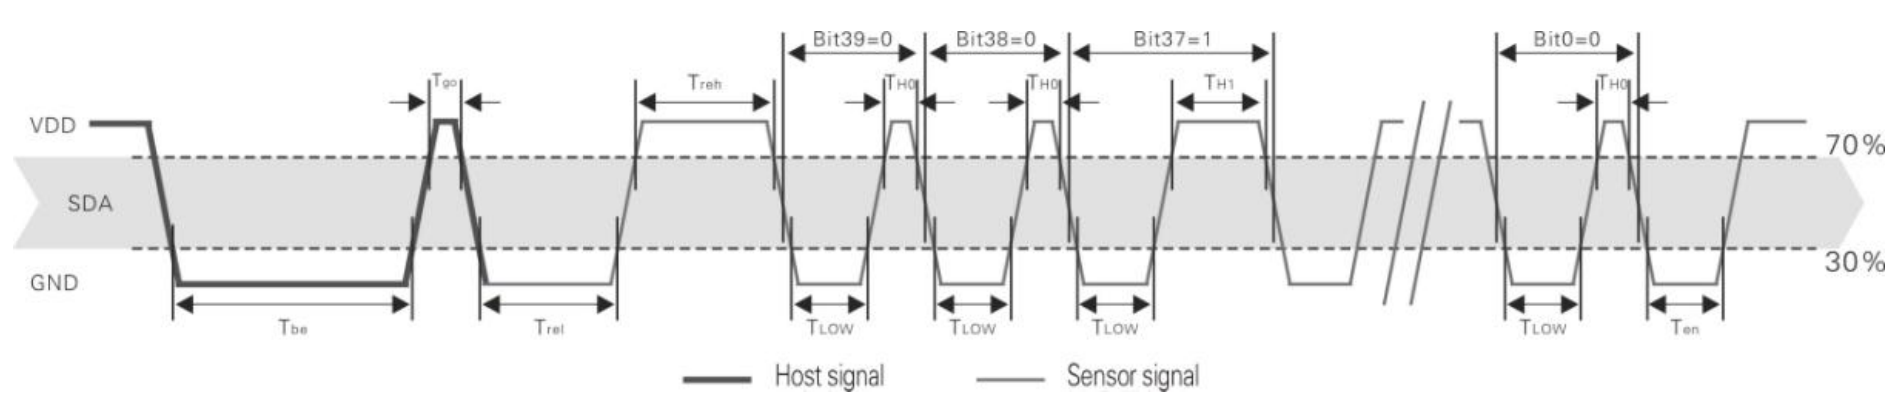
\includegraphics[width=1.1\textwidth]{./Bilder-Tobit/one-wire-protokoll.PNG}
    \caption{Übertragungsprotokoll des AM2302 (ONE-WIRE)}
    \label{fig:ONE-WIRE}
\end{figure}

Der gesamte Datensatz wird über diese Kodierung übertragen.\\
Ein Datensatz umfasst 40 Bits,
die zwei oberen Bytes stellen dabei die Luftfeuchtigkeit dar, Byte 3 und 4 beschreibt die Temperatur und das 5 Byte wird für Parität genutzt;
zur Gültigkeit des Datensatzes muss die Addition aus den ersten vier Bytes das Paritätsbyte ergeben.\\

Anhand dieser Erkenntnisse wurde zunächst ein Testprojekt erstellt, in dem grundlegende Operationen getestet wurden.

\subsubsection{Sensor auslesen}
\label{sec:sensor_auslesen}
Zu Beginn wurde zunächst ein Test durchgeführt, welcher dem Sensor ein einfaches Startsignal schickt, um das senden eins Datensatzes zu triggern.\\

Dazu wurde ein Pin auf \textit{Low} gesetzt. Anschließend für 18ms gewartet und danach auf Input umgestellt.\\
Die Umstellung auf \textit{Input} bewirkt, dass der Pin in einen \textit{Hochohmigen} Zustand gesetzt wird, in dem er neutral im Stromkreis ist.
Durch den PullUp-Widerstand, der auf der Sensor-Platiene schon angebracht ist, ändert der Pegel auf \textit{High}.\\
Mit Hilfe eines Logic Analyzer konnte dann der darauffolgende Datensatz (siehe \cref{fig:startsignal} ) manuell entziffert
und in Luftfeuchtigkeit und Temperatur umgerechnet werden,
ebenso konnte auch das Paritätsbyte dieses Datensatzen verifiziert werden.\\

Hier der entsprechende Commit\footnote{\url{https://gitlab.rz.htw-berlin.de/s0582020/ce31-embd-gruppe-6-tz-kh/-/blob/b6c98919b875442ec13493a7b8098ecf4a4c31c1/Tobit/test-pr/Core/Src/_main2.c}}.\\

\begin{figure}[H]
    \centering
    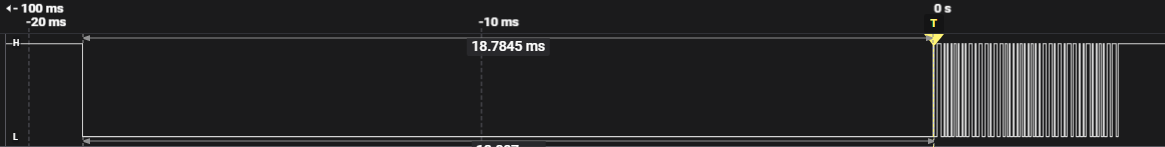
\includegraphics[width=\textwidth]{./Bilder-Tobit/send_startsignal.PNG}
    \caption{Senden eines Startsignals und Werte vom Sensor}
    \label{fig:startsignal}
\end{figure}

\subsubsection{Erfassung von Sensordaten}
Nach erfolgreicher triggern der Datenbereitstellung durch den Sensors,
wurde im anschließenden Schritt mit der Erfassung und Speicherung der Daten durch den Mikrocontroller begonnen.\\

Da die Einsen und Nullen nicht über Spannungspegel definiert sind, sondern über die zeitliche Länge des High-Pegels,
wurde für diese Aufgabe ein \textit{Hardware-Timer} eingesetzt.
\footnote{Alle benötigten Informationen zum Einrichten und Auslesen von Timern wurden aus Laboraufgaben
    aus früheren Semestern entnomen.}
Dieser Timer (oder dt. Zähler) startet, sobald eine Flanke (zunächst steigend oder fallend) am Datenbus anliegt.
Bei einer folgenden Flanke wird der Zählerwert in einen \textit{Puffer} gespeichert und der Zähler zurück auf Null gesetzt.\\
Der Timer zählt mit einer Geschwindigkeit von 1MHz (Clock speed: 32 MHz und Prescaler: 32).
Das Timer-Register hat 16 Bit, der Timer kann also etwa für 65ms Zählen, bis es zu einem Überlauf des Registers kommt.
Die Größe des Registers ist somit außreichend groß.\\

An der Stelle, an welcher im \cref{sec:sensor_auslesen} das GPIO auf Input-Mode gestellt wurde,
wurde in diesem Abschnitt ein Pin auf \textit{External Interrupt Mode with Rising/Falling edge trigger detection} gestellt.\\
Damit können alle Flankenänderungen recourcensparend und zuverlässig behandelt werden.
Ein Pin (oder GPIO) in solch einem Modus ist (wie ein Pin im Input-Modus) hochohmig und dadurch neutral im Stromkreis.

Nach Ausführung des Programms
\footnote{Hier der entsprechende Commit: \url{https://gitlab.rz.htw-berlin.de/s0582020/ce31-embd-gruppe-6-tz-kh/-/blob/7e12f31a90cf9912a9331d4b3186aa174c0ed062/Tobit/test-pr/Core/Src/main.c}}
im \textit{Debug-Modus} konnten die Werte aus dem Puffer (siehe \cref{fig:Puffer_1}) mit den Werten des Logic Analyzers (siehe \cref{fig:Puffer_LA_1}, \cref{fig:Puffer_LA_2}, \cref{fig:Puffer_LA_3}) verglichen werden
und folgende Schlüsse gezogen werden:
\begin{itemize}
    \item Das erste und zweite Element (0 und 13) sind kein Bestandteil des eigentlichen Datensatzes;
          beide sind in jedem Datensatz enthalten der bisher getestet wurde.
    \item Die 13 (buf[1]) entsteht vermutlich daher, weil von dem Zeitpunktes des Timer-Start bis zur ersten steigenden Flanke schon Zeit verstrichen ist.
    \item Die gepufferten Zeiten sind immer etwas kleiner (4 bis 6µs), als die gemessenen Zeiten des Logic Analyzers:\\
          Im Puffer steht z.B. der Wert 18, gemessen wurde allerdings 22µs (siehe \cref{fig:Puffer_LA_1})
          oder gesessen 78µs (siehe \cref{fig:Puffer_LA_2}) und im Puffer steht 72µs
          oder es steht im Puffer 22µs aber es wurden 26µs (\cref{fig:Puffer_LA_3}) gemessen.\\
          Vermutlich entsteht dieses Phenomen durch den zeitlichen Versatz des Auslesens vom Timerwert und dem zurücksetzen des Wertes auf 0.\\
          Allerdings ist dieses Problem ohne Bedeutung, da die Unterschiede zwischen gemessener und gepufferter Zeit noch gut in der Tolleranz liegen.
\end{itemize}

\begin{figure}[H]
    \centering
    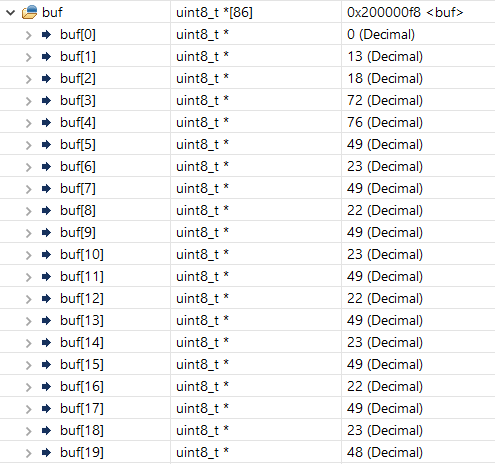
\includegraphics[width=0.6\textwidth]{./Bilder-Tobit/Datenerfassung_pufferausschnitt.PNG}
    \caption{Erfassen der Zeitlängen; Pufferausschnitt}
    \label{fig:Puffer_1}
\end{figure}

\begin{figure}[H]
    \centering
    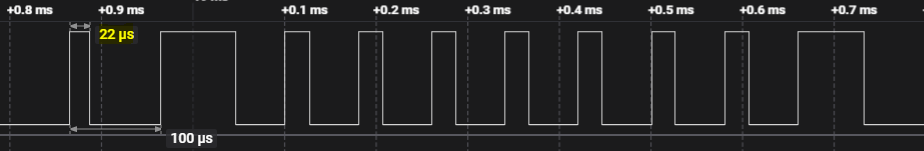
\includegraphics[width=\textwidth]{./Bilder-Tobit/Datenerfassung_LA_1.PNG}
    \caption{1. Beispiel gemessener Zeiten, Logic Analyzer}
    \label{fig:Puffer_LA_1}
\end{figure}

\begin{figure}[H]
    \centering
    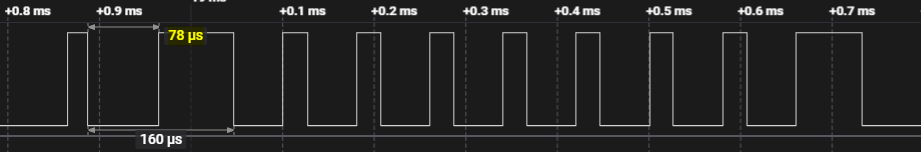
\includegraphics[width=\textwidth]{./Bilder-Tobit/Datenerfassung_LA_2.PNG}
    \caption{2. Beispiel gemessener Zeiten, Logic Analyzer}
    \label{fig:Puffer_LA_2}
\end{figure}

\begin{figure}[H]
    \centering
    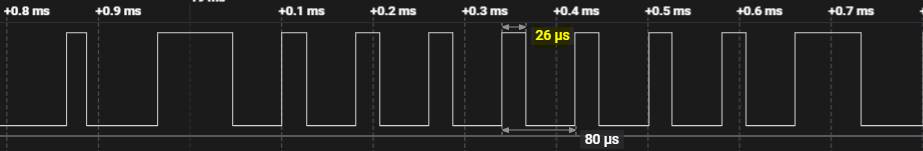
\includegraphics[width=\textwidth]{./Bilder-Tobit/Datenerfassung_LA_3.PNG}
    \caption{3. Beispiel gemessener Zeiten, Logic Analyzer}
    \label{fig:Puffer_LA_3}
\end{figure}

\subsubsection{Messen der \textit{High} Zeitlängen}
\label{sec:messen_zeitleangen}
Bisher wurden alle Zeitlängen, also Verschrichene Zeit im Low Pegel und im High Pegel, im Puffer gespeichert.
Die Daten werden allerdings nur über die zeitliche Länge des High-Pegels definiert (Kurzer High Pegel: 0, langer High Pegel: 1).\\
In diesem Schritt wurde zum herausfiltern der Low Zeiten, dazu die \textit{Interrupt service routine (ISR)} angepasst.\\

Vorher wurde bei \textbf{jeder} Flanke die Zeit abgelesen, im Puffer gespeichert und der Timer zurückgesetzt,
hier wird bei jeder \textbf{steigenden} Flanke der Zähler gestartet (Anfang einer High-Phase) und
bei einer \textbf{fallenden} Flanke (High-Phase beendet) die verstrichene Zeit abgespeichert und der Timer auf 0 zurückgesetzt.

Um die jeweilige Flanke zu erkennen wird über \textit{if-Abfragen} der Pegel getestet.
Ist der anliegende Pegel High, so trat eine steigende Flanke auf und wenn der anliegende Pegel Low ist, lag eine fallend Flanke vor.
\footnote{Hier der zugehörige Commit: \url{https://gitlab.rz.htw-berlin.de/s0582020/ce31-embd-gruppe-6-tz-kh/-/blob/14fc2910820f579252b00a05db28e5292ac06d0a/Tobit/test-pr/Core/Src/main.c}}

Im folgenden der Pufferausschnitt, wenn alle Low-Phasen herausgefiltert sind (siehe \cref{fig:Puffer_zeitleangen}).
\begin{figure}[H]
    \centering
    \includegraphics[width=0.6\textwidth]{./Bilder-Tobit/Zeitlängen_pufferausschnitt.PNG}
    \caption{Messen der High Zeitlängen; Pufferausschnitt}
    \label{fig:Puffer_zeitleangen}
\end{figure}

In diesem Schritt ist die führende Null nun nicht mehr vorhanden.\\

Das folgende Bild veranschaulicht, wie die 12µs zustande kommen (siehe \cref{fig:Flanken}),
obwohl diese nicht zum eigentlichen Datensatz gehören.\\
Nach dem der Timer startet, wird zunächst noch der Interrupt für das Pin konfiguriert.
Anschließend wird die steigende Flanke erkannt, welche den Timer zurücksetzt
und daraufhin die fallende Flanke, welche den Timerwert abspeichert.
Diese 14.5µs entsprechen der 12, welche in den Puffer geschrieben wurde.

\begin{figure}[H]
    \centering
    \includegraphics[width=\textwidth]{./Bilder-Tobit/Zeitlängen_LA_1.PNG}
    \caption{Flankenerkennung des Nucleos}
    \label{fig:Flanken}
\end{figure}

Mit diesen Ergebnissen kann nun der erste Schritt, die Sensordaten auslesen und abspeichern, abgeschlossen werden.\\
Die Daten aus dem Puffer müssen nur noch zwischen lang (entspricht einer 1) und kurz (entspricht einer 0) aufgeteilt werden.\\

\subsubsection{Timeouts erkennen}
\label{sec:Timeouts_erkennen}
Mit dem vorangegangenen Abschnitt wurde das lesen eines Datensatzes im \textit{Happy-Day-Szenario} beendet,
das heißt, das lesen des Datensatz verläuft ohne Zwischenfälle.\\
In diesem Abschnitt wurde während des Entwicklungsprozesses der Fall betrachtet, wenn die Übertragung abbricht,
das heißt: nicht alle 40 Bits sind vollständig.

Dazu wurde der Timer als ausschlagebendes Kriterium genutzt.
\footnote{Hier der zugehörige Commit: \url{https://gitlab.rz.htw-berlin.de/s0582020/ce31-embd-gruppe-6-tz-kh/-/blob/802b78e46e3046979759920bed217532faf7c814/Tobit/test-pr/Core/Src/main.c}}
Grundsätzlich wird bei jeder steigenden Flanke der Timer auf Null zurückgesetzt.
Das Zurücksetzen verhindert somit das Überlaufen des Timer-Registers.
Die Idee: wenn der Timer überläuft, kam keine steigende Flanke, die den Timer zurückgesetzt hätte und so den Überlauf verhindert.
Da allerdings der Timer im hypotetischen Fall übergelaufen ist, liegt ein Fehler vor.\\

Somit kann das Überlaufen als notwendiges Kriterium angesehen werden, Timeouts während der Übertragung festzustellen.\\

Einen Timerüberauf wird am Besten mithilfe eines Interrupts ermittelt.
Da allerdings der bisher genutzte Timer nicht den globalen Interrupt unterstützt hatte,
wurde zu einem anderen Timer (nun TIM7) gewechselt.
Abgesehen von der Interruptaktivierung wurde zusätzlich noch die Periodenlänge auf 200µs reduziert.
Aufgrund dieser Reduzierung zählt der Timer nun nur noch bis maximal 200, wodurch es schneller zu einem Überlauf kommt.
Der Vorteil davon ist, dass nun schneller auf das Timeout reagiert werden kann.

Hier gab es allerdings das Problem, dass immer direkt nach dem Starten des Timer-Interrupts der Interrupt auslöste.
Auf stackoverflow wurde dafür jedoch eine Lösung gefunden.
\footnote{\url{https://stackoverflow.com/questions/71099885/why-hal-tim-periodelapsedcallback-gets-called-immediately-after-hal-tim-base-sta}}

Wie im folgenden Bild (\cref{fig:tim_int}) ersichtlich, scheint diese Methode ein aussagekräftiges Kriterium darzustellen,
um ein unerwartetes Beenden der Übertragung festzustellen.
Denn bei jeder steigenden Flanke wird der Timer auf Null zurückgesetzt (entspricht einem Toggeln des orangenen Pegels).
Nach der letzten steigenden Flanke des Datensatzes tritt nach etwas mehr als 200µs eine Pegeländerung (im Bild orange dargestellt) auf,
diese ist dem Auslösen des Interruptes zuzuscheiben (siehe Quellcode).
Im Falle eines tatsächlichen Abbruchs würden an dieser Stelle Maßnahmen ergriffen.

\begin{figure}[H]
    \centering
    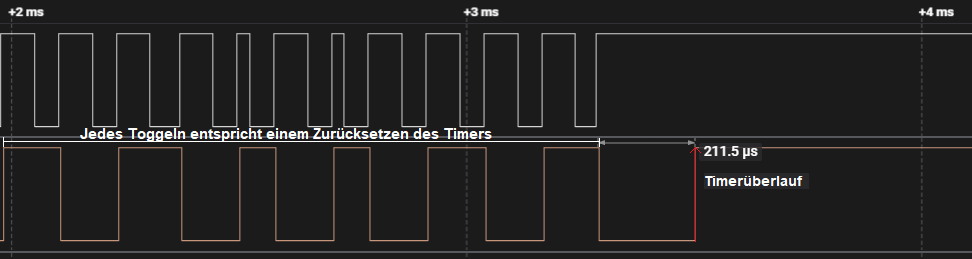
\includegraphics[width=\textwidth]{./Bilder-Tobit/timer_interrupt_1.PNG}
    \caption{Timer Interrupt}
    {\small oben: Übertragung des Datensatzes, unten: jedes zurücksetzen des Timers ist ein Togglen des Pegels}
    \label{fig:tim_int}
\end{figure}

\subsubsection{Masterseitiges I²C}
\footnote{Im folgenden der entsprechende Commit: \url{https://gitlab.rz.htw-berlin.de/s0582020/ce31-embd-gruppe-6-tz-kh/-/blob/51545de28ded9a42c2e88143d0d02d6806328ec1/Tobit/test-pr/Core/Src/main.c}}
Ein letzter wichtiger Punkt, der noch zu testen gilt, stellt die Übertragung der Daten auf das zweite Nucleo-Board dar.\\
In diesem Projeckt wurde eine I²C basierte Kommunikation gewählt.
Die masterseitige I²C Kommunikation wurde in diesem Abschnitt des Erarbeitungsprozesses ausgetestet.\\

Um die Übertragung aussagekräftig Überprüfen zu können,
wurde an dieser Stelle ein weiterer Mikrocontroller benötigt, um die Slave-Seite zu simulieren.\\
Da dem Entwickler allerdings kein zweites Nucleo-Board verfügbar war,
wurde als Alternatieve hier ein Arduino NANO EVERY eingesetzt.\\

Auf Seiten des Arduinos wurde die Standardsoftware \textit{slave\_receiver} aus der \textit{wire-Library} genutzt,
um alle ankommenden Daten über den \textit{Serial Monitor} auszugeben.

Für den Nucleo wurde im Codegerüstgenerator das I2C1-Interface aktiviert.\\
An diesen Punkt wurde sich mit dem Kollegen (siehe \cref{sec:7-seg-anzeige}) auf folgende Schnittstelle geeinigt:
Standart-Geschwindigkeit (100 KHz) und 7-Bit Adressen.
\footnote{Eine detailiertere Schnittstellenbeschreibung unter: \url{https://gitlab.rz.htw-berlin.de/s0582020/ce31-embd-gruppe-6-tz-kh/-/blob/main/README.md}}
\\

Als PullUp Widerstände werden zwei 2KOhm Widerstände eingesetzt,
die Anstiegsflanke wurde mittels Osziloskop gemessen (siehe \cref{fig:oszi_rising_falling_edges}).\\
Anhand des Bildes scheint es, dass 2kOhm ein guter Kompromiss zwischen Anstiegszeit (etwa 1µs) und Stromverbrauch ($I\,=\,\frac{3v3}{2\,kOhm}\,\approx\,1\,mA$) ist.

\begin{figure}[H]
    \centering
    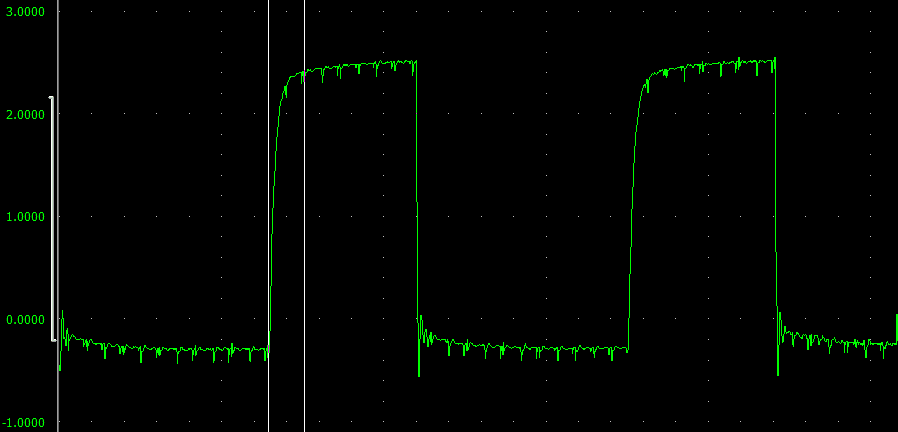
\includegraphics[width=\textwidth]{Bilder-Tobit/oszi_rising_falling_edges_1.png}
    \caption{Messung der Anstiegsdauer bei 2KOhm PullUp Widerstand}
    {\small zwischen den beiden Cursor liegt 1µs}
    \label{fig:oszi_rising_falling_edges}
\end{figure}

Im folgenden der I²C-Testaufbau (siehe \cref{fig:i2c_testaufbau}).

\begin{figure}[H]
    \centering
    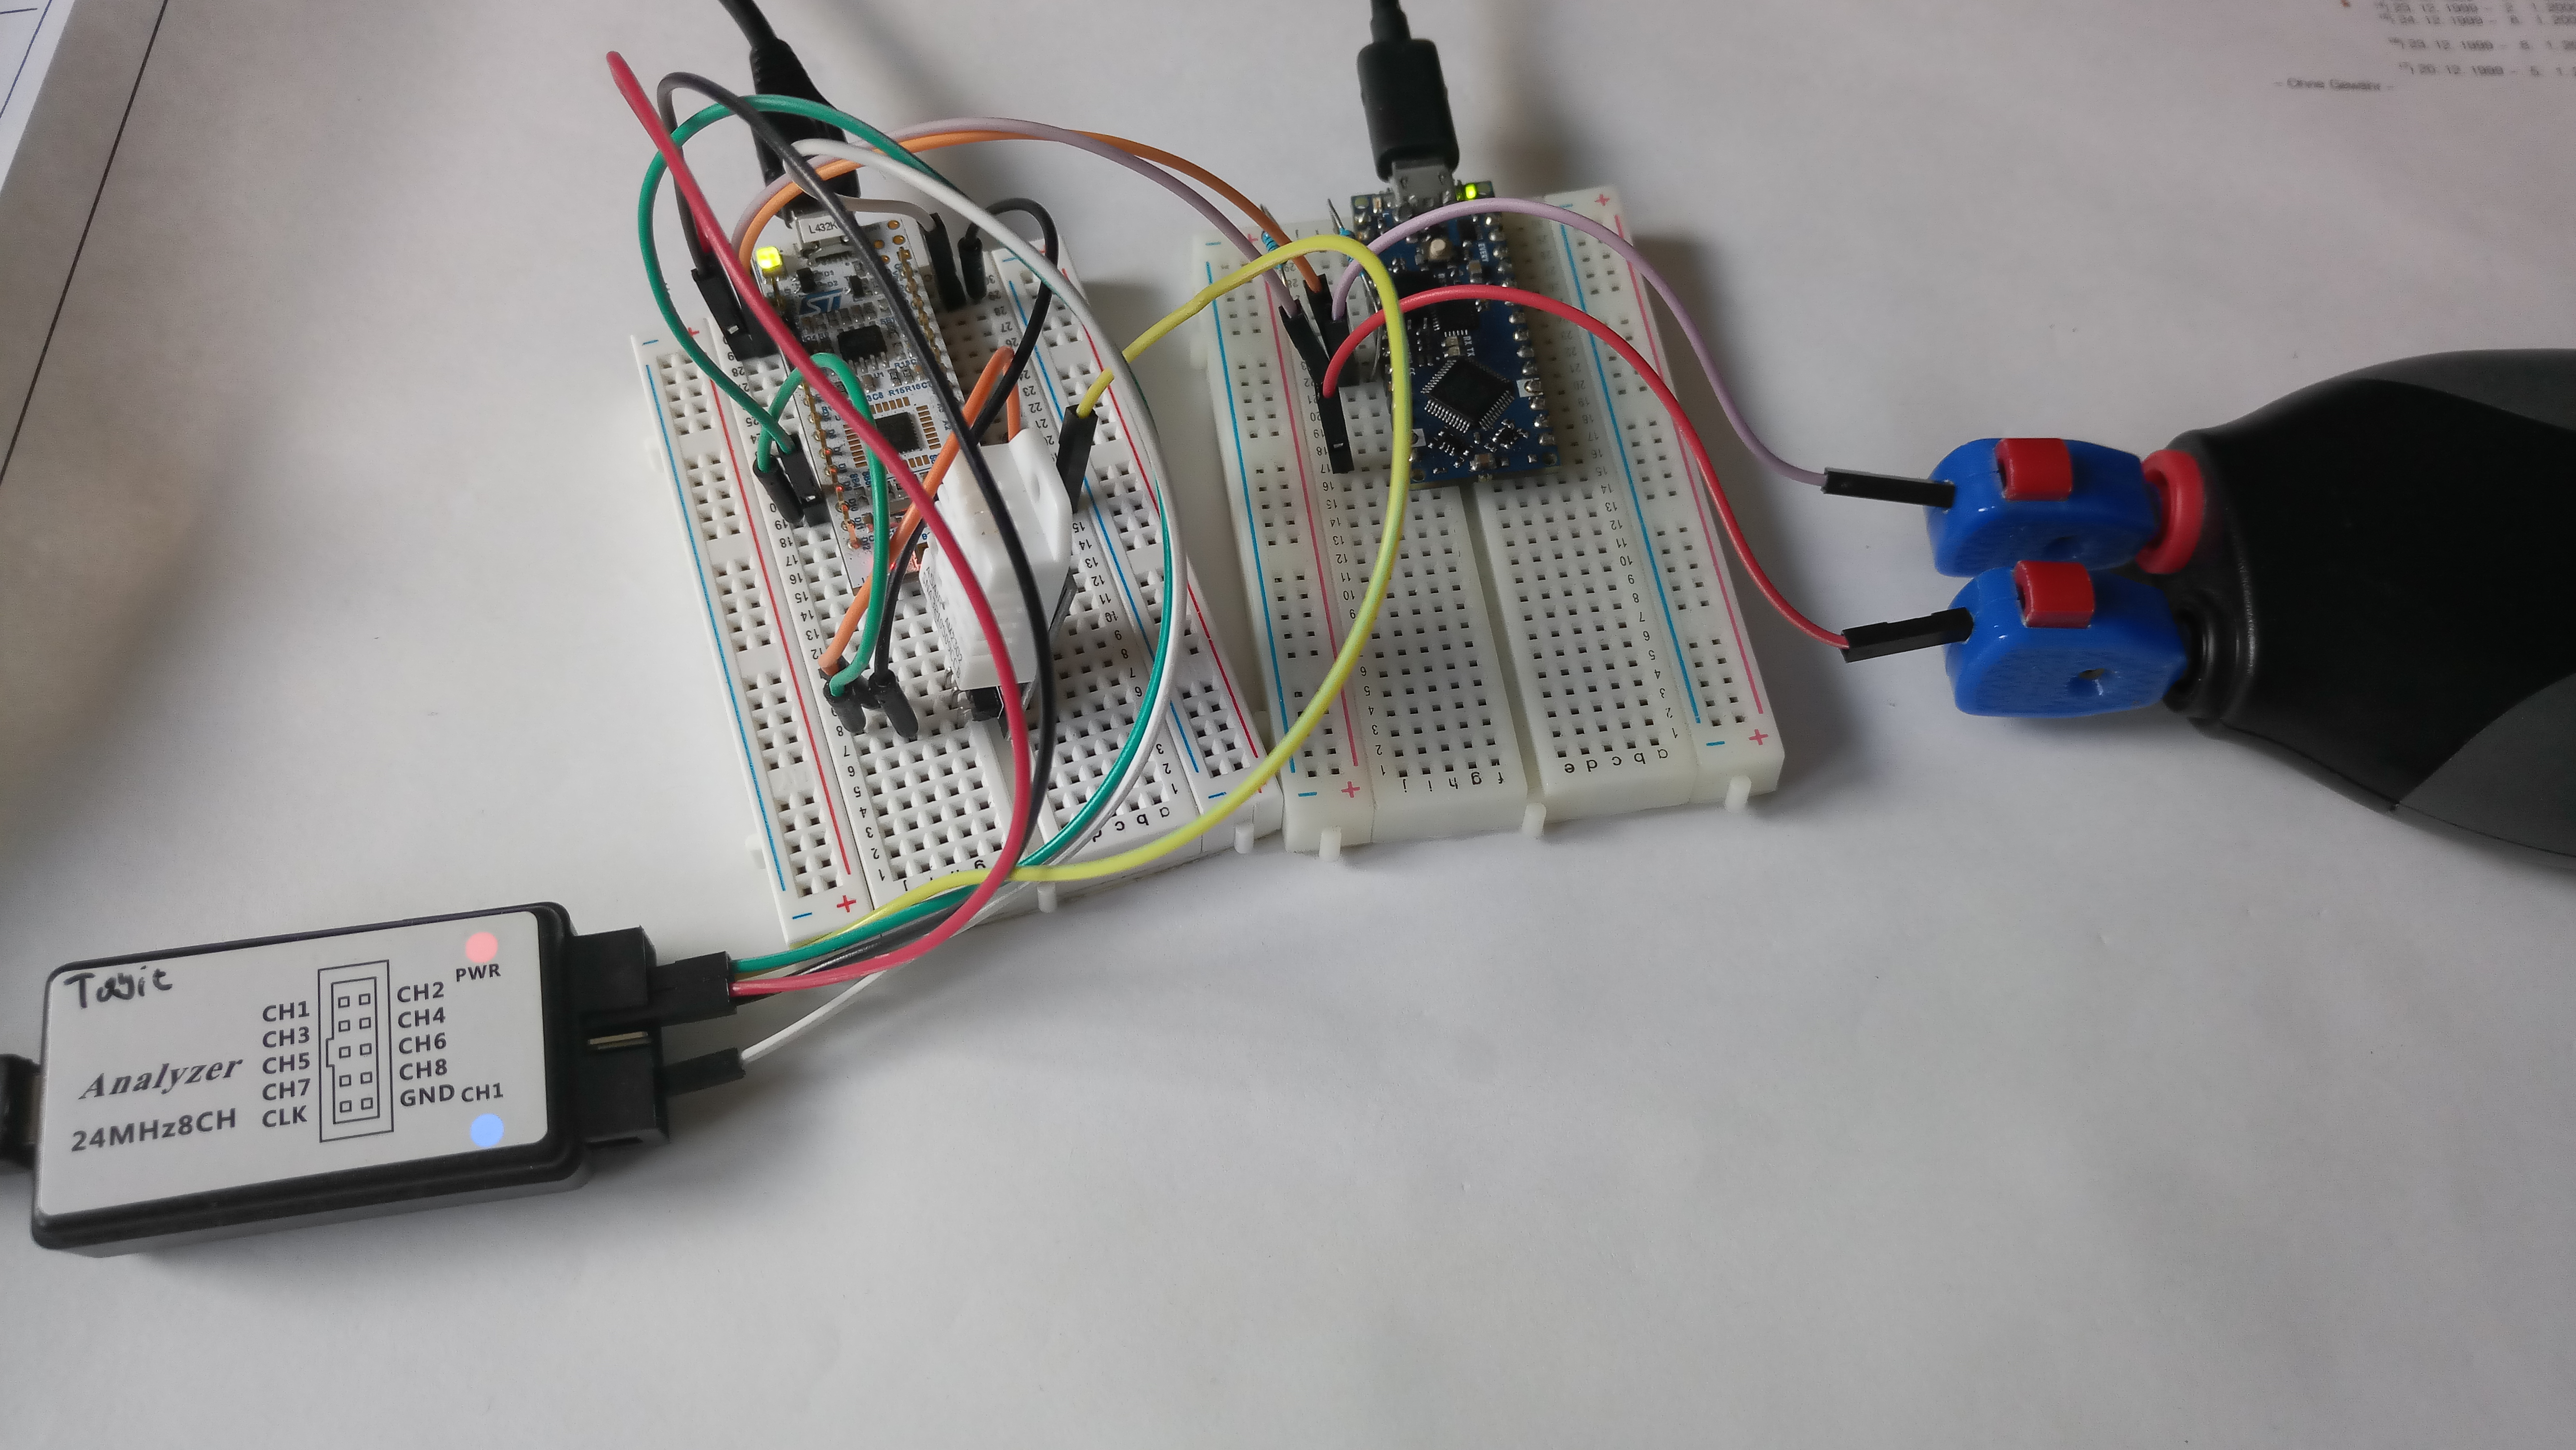
\includegraphics[width=\textwidth]{./Bilder-Tobit/i2c_testaufbau.jpg}
    \caption{Testaufbau I²C}
    {\small links: Nucleo als Master, rechts: Arduino als Slave}
    \label{fig:i2c_testaufbau}
\end{figure}

Als I²C-Test wurde unter anderem ein Array aus 4 \textit{uint16\_t} Elementen übertragen (siehe \cref{fig:i2c_test_transmission}).

\begin{figure}[H]
    \centering
    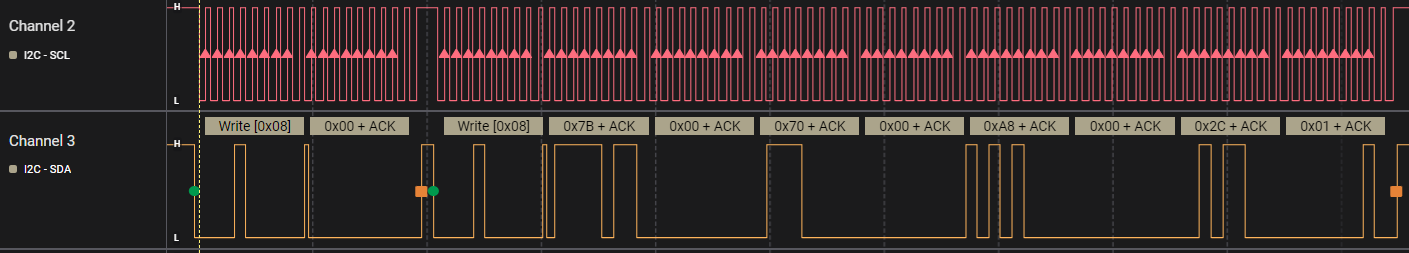
\includegraphics[width=1.1\textwidth]{./Bilder-Tobit/i2c_test_transmission.jpg}
    \caption{Beispielübertragung einer 0 und des Arrays \texttt{test[]=\{123,112,168,300\};}}
    \label{fig:i2c_test_transmission}
\end{figure}

Ein Problem trat allerdings dabei auf: Um den Slave mit der Adresse 8 anzusprechen,
war es nötig 16 als Adresse anzugeben, also das Doppelte bzw. ein Bitschift nach links.\\

Mit dem erfolgreichen Senden von Beispieldaten konnten die vorbereitenden Test abgeschlossen und die finale Entwicklung gestartet werden.

\subsubsection{Projekt Implementierung}

Um eine struckturierte und logische Implementierung anfertigen zu können, wurde zunächst ein \textit{Flussdiagramm} angefertigt,
welches im laufe der Erarbeitung an einigen Stellen nachgebessert wurde.\\

Die Grundstrucktur ist eine Zustandsmaschine mit sechs Zuständen: \textit{ready, measuring, finished, processing, invalid} und \textit{error}.
Der Initialzustand ist dabei \textit{ready}.\\

Das System beginnt mit einem StartUp (siehe \cref{fig:flussdiagramm_main}), in welchem unter anderem die I²C Verbindung überprüft wird.
Der Master-Nucleo sendet dabei einen Konstanten Wert an den Slave-Nucleo, welcher wiederum mit einem vordefinierten Wert reagiert.
Damit wird sowohl eine bestehende Verbindung verifiziert,
aber es dient auch zur Authentifizierung des Slaves.\\

Kommt das System durch den StartUp, folgt die \textit{Hauptschleife}.\\
In der \textit{Hauptschleife} rotiert das System dauerhaft (ohne Abbruch) und überprüft, auf welchen Zustand das System gesetzt wurde.
Abhängig vom Zustand wird dann die entsprechende Funktion aufgerufen.\\

Der \textbf{ready}-Zustand (siehe \cref{fig:flussdiagramm_main}) gibt die Freigabe um eine Messung durchzuführen.
Hierbei wird zunächst überprüft, ob die vorangegangene Messung älter als 2 Sekunden ist, da sonst der Sensor fehlerhafte Daten ausgibt.\\
Ist die vorangegangene Messung tatsächlich älter als 2 Sekunden, wird der Status auf \textbf{measuring} gesetzt.
Nun folgt das Senden eines Startsignal, wie es zuvor im Test-Projekt geschehen war (\cref{sec:sensor_auslesen}).
Das Aktiviren der Interruptes (Timer und GPIO) und das Setzen des Status \textit{measuring},
sind die Türöffner für den eigentlichen Prozess des Einlesens des Datensatzes.
\footnote{Dieser Prozess wurde bereits im Abschnitt \cref{sec:messen_zeitleangen} erläutert.}
(siehe \cref{fig:flussdiagramm_ISR}).\\
Potentielle Fehlerfälle (Überschreiten von Zeittolleranzen oder die Anzahl der Bits)
werden mit dem entsprechenden Statuswechsel signalisiert und in der nächsten Hauptschleife bearbeitet.\\
Beispielsweise sorgt das Verbleiben einer Datenflanke während eines Datensatzes das Überlaufen des \textit{TIM7}-Registers.
Aus diesem Ereignis lässt sich schließen, dass wahrscheinlich keine Verbindung zum Sensor besteht (siehe \cref{sec:Timeouts_erkennen}),
weswegen die Statusvariable auf Error 2 gesetzt wird.
Dieser Error-Code steht für ``Keine Verbindung vom Sensor''.\\

Bei erfolgreichem Lesen und Abspeichern des empfangenen Datensatzes wird schließlich auch die Statusvariable auf \textit{finished} umgestellt.\\

Mit dem Status \textbf{finished} (siehe \cref{fig:flussdiagramm_finished}) werden die jüngst empfangenen Zeitwerte
in Bits umgerechnet (siehe \cref{sec:messen_zeitleangen}) und validiert.
Anders als im Zustand \textit{measuring}, werden hier die Zeitlängen der einzelnen Bits und das Paritätsbyte überprüft.
Im Fehlerfall wird der Zustand auf \textit{invalid} gesetzt.\\

Nach erfolgreicher Validierung blockiert das System nun und wartet solange, 
bis 5 Sekunden seit der letzten Datenübertragung zum Slave vergangen sind.

Anschließend folgt das Senden der Daten; es wird abwechselnd die Luftfeuchtigkeit oder die Temperatur gesendet.
Ebenso wird der \textit{invalid-Zähler}, welcher die Anzahl der bisher aufgetretenen invalid-Zustände speichert, zurückgesetzt
und der Zustand wieder auf \textit{ready} gesetzt, um den nächsten Datensatz zuerfassen.\\

Trat der Zustand \textbf{invalid} (siehe \cref{fig:flussdiagramm_invalid_error}) auf,
wird zunächst über das Eintreten des invalid-Zustands mit der \textit{Statusled} informiert.
Der \textit{invalid-Zähler} wird inkrementiert.
Trat dieser Zustand schon zuhäufig auf, wird der Fehlercode 3 über I²C gesendet und auf der Sieben-Segment-Anzeige dargestellt.
Der invalid-Zähler wird erst bei einem erfolgreichen \textit{processing} zurückgesetzt.
Am Ende dieses Zustands wird die Statusvariable auf \textit{valid} gesetzt, um erneut eine Messung zu versuchen.\\

Auch im \textbf{error}-Zustand wird der entsprechende Fehlercode über die Statusled angezeigt, allerdings über ein anderes Blinksignal.
Wenn eine Verbindung zum Nucleo mit Sieben-Segment-Anzeige besteht, wird auch hier der Fehlercode übertragen.
Da es sich bei Fehlercode 1 und 2
\footnote{Code 1 steht für keine Verbindung zum I²C-Slave und Code 2 steht für keine Verbindung zum Sensor.}
um Fehler handelt, die nicht unbedingt durch das erneute versuchen einer Messung gelöst werden können,
wird beim Error-Status der Nucleo \textit{rebootet}.\\

\begin{figure}[H]
    \centering
    % \includesvg[width=\textwidth]{./Bilder-Tobit/flussdiagramm_main.svg}
    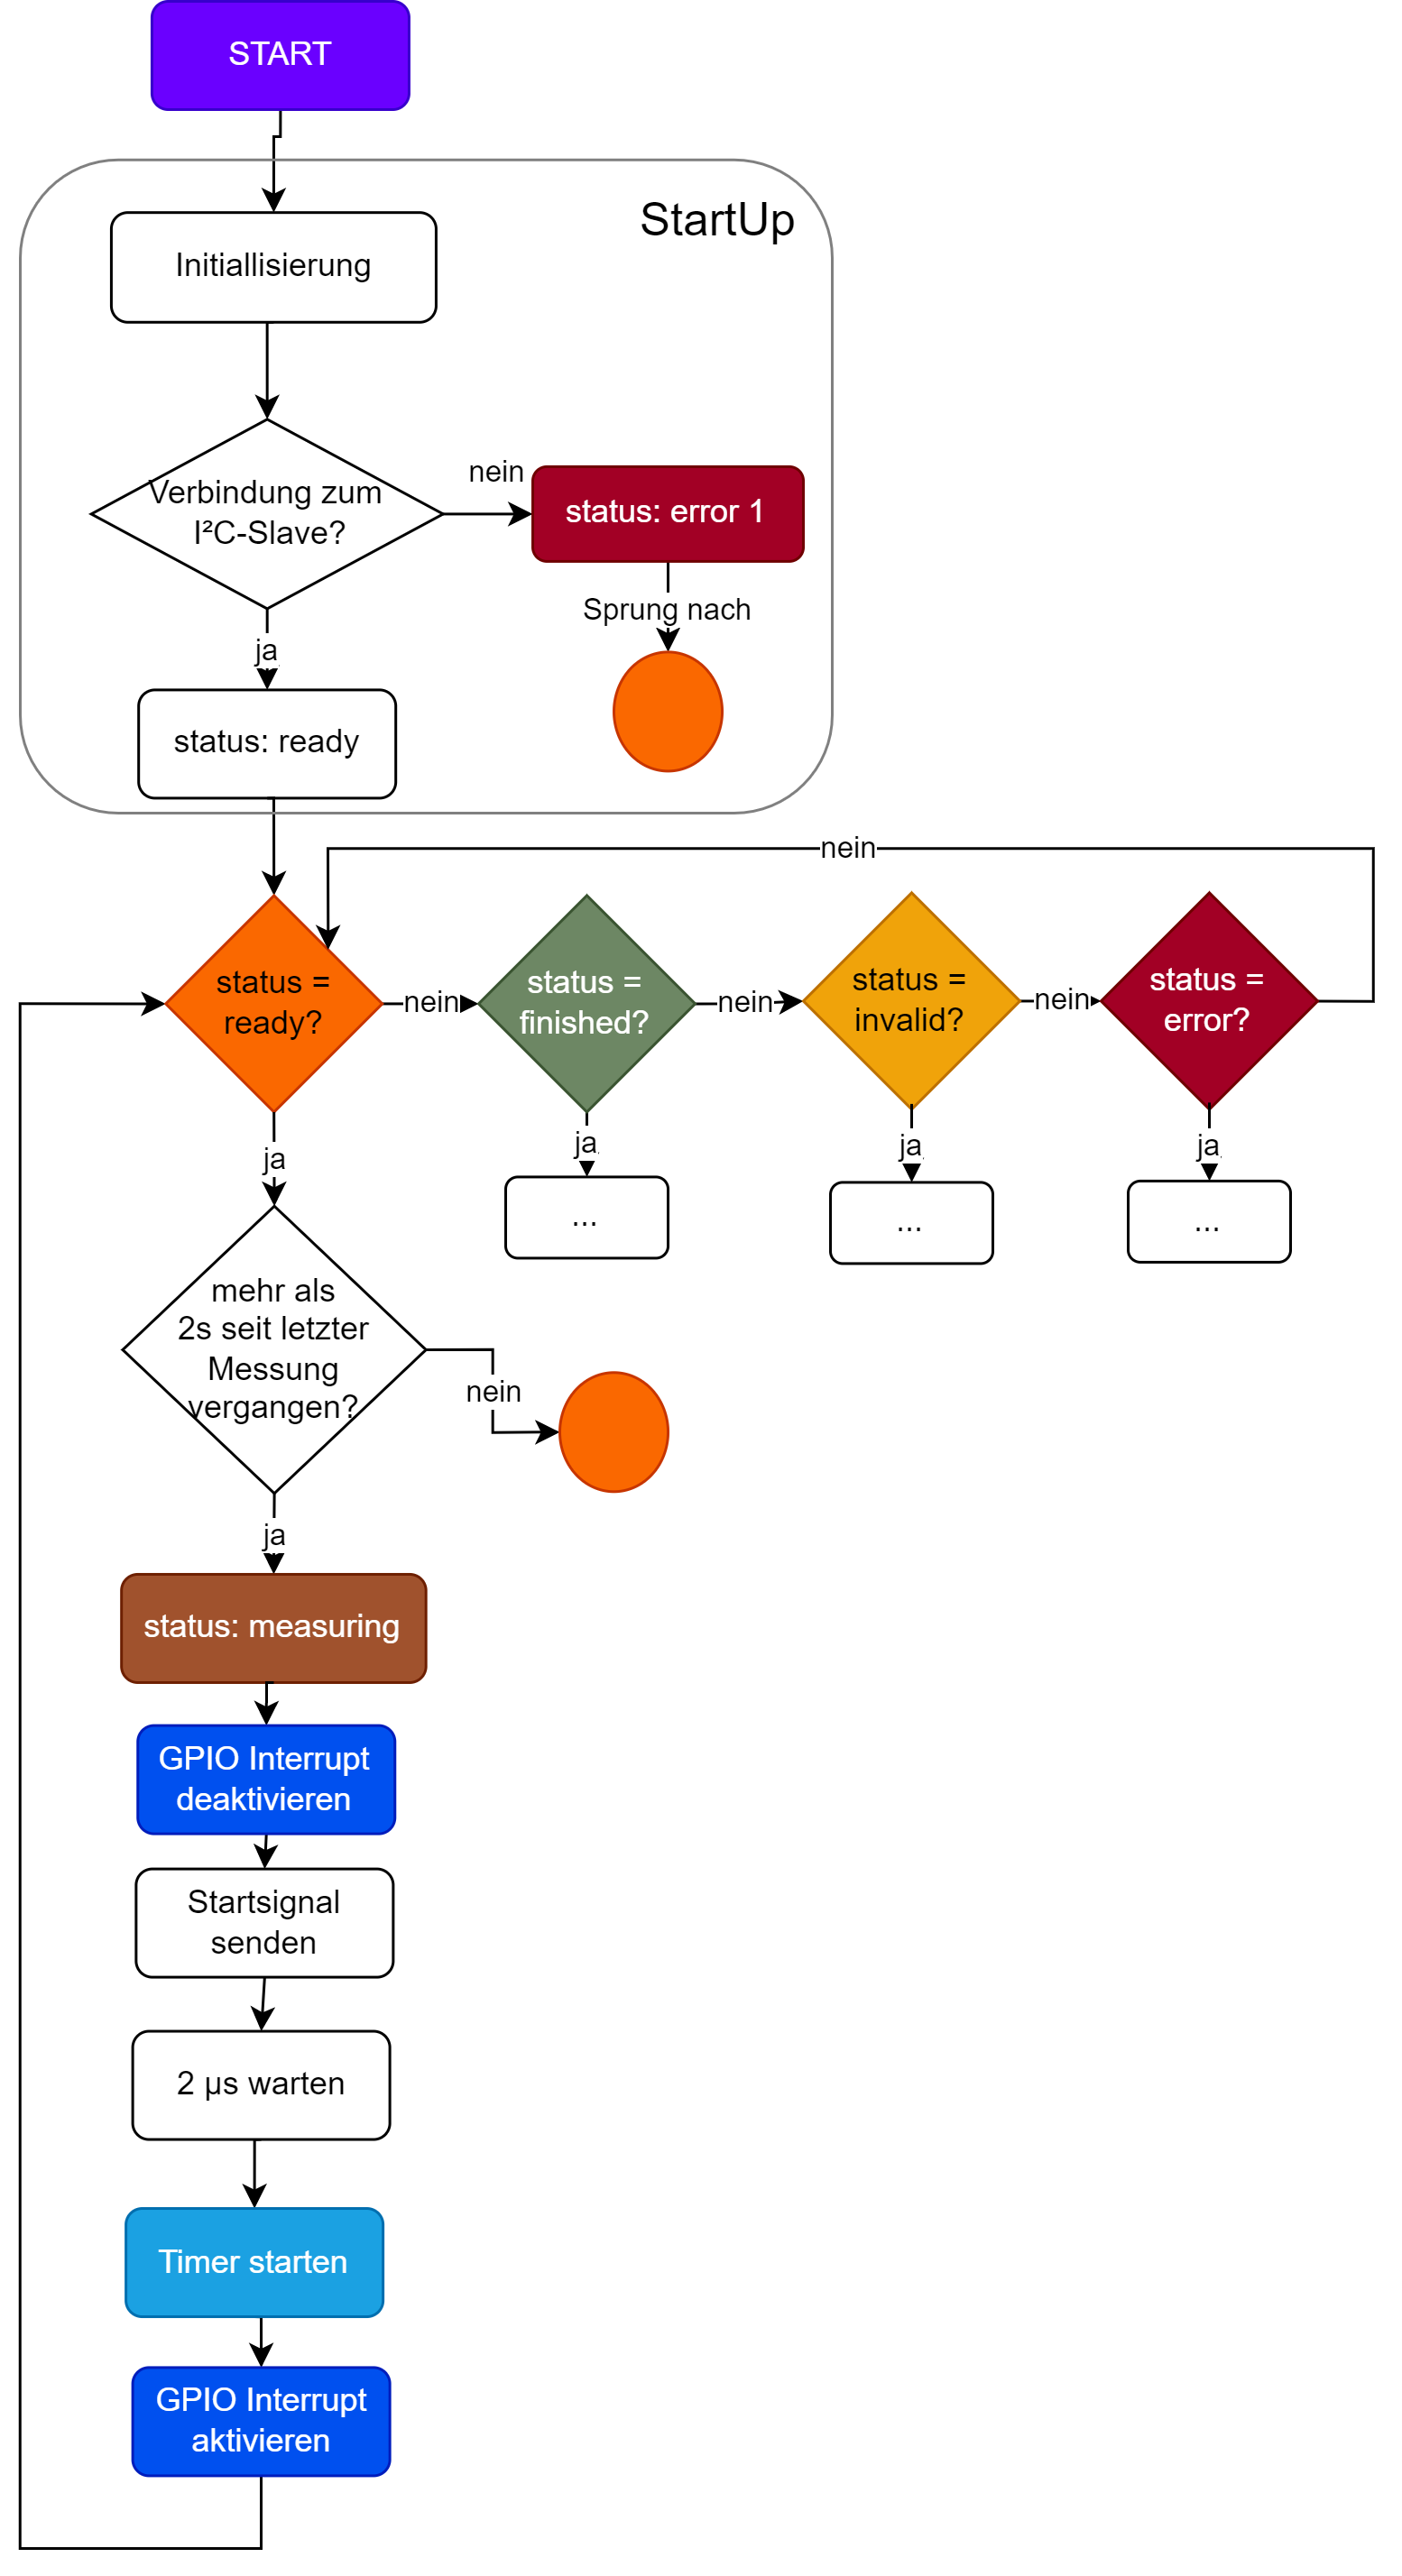
\includegraphics[height=0.9\textheight]{./Bilder-Tobit/flussdiagramm_main.png}
    \caption{Flussdiagramm: Hauptschleife}
    \label{fig:flussdiagramm_main}
\end{figure}

\begin{figure}[H]
    \centering
    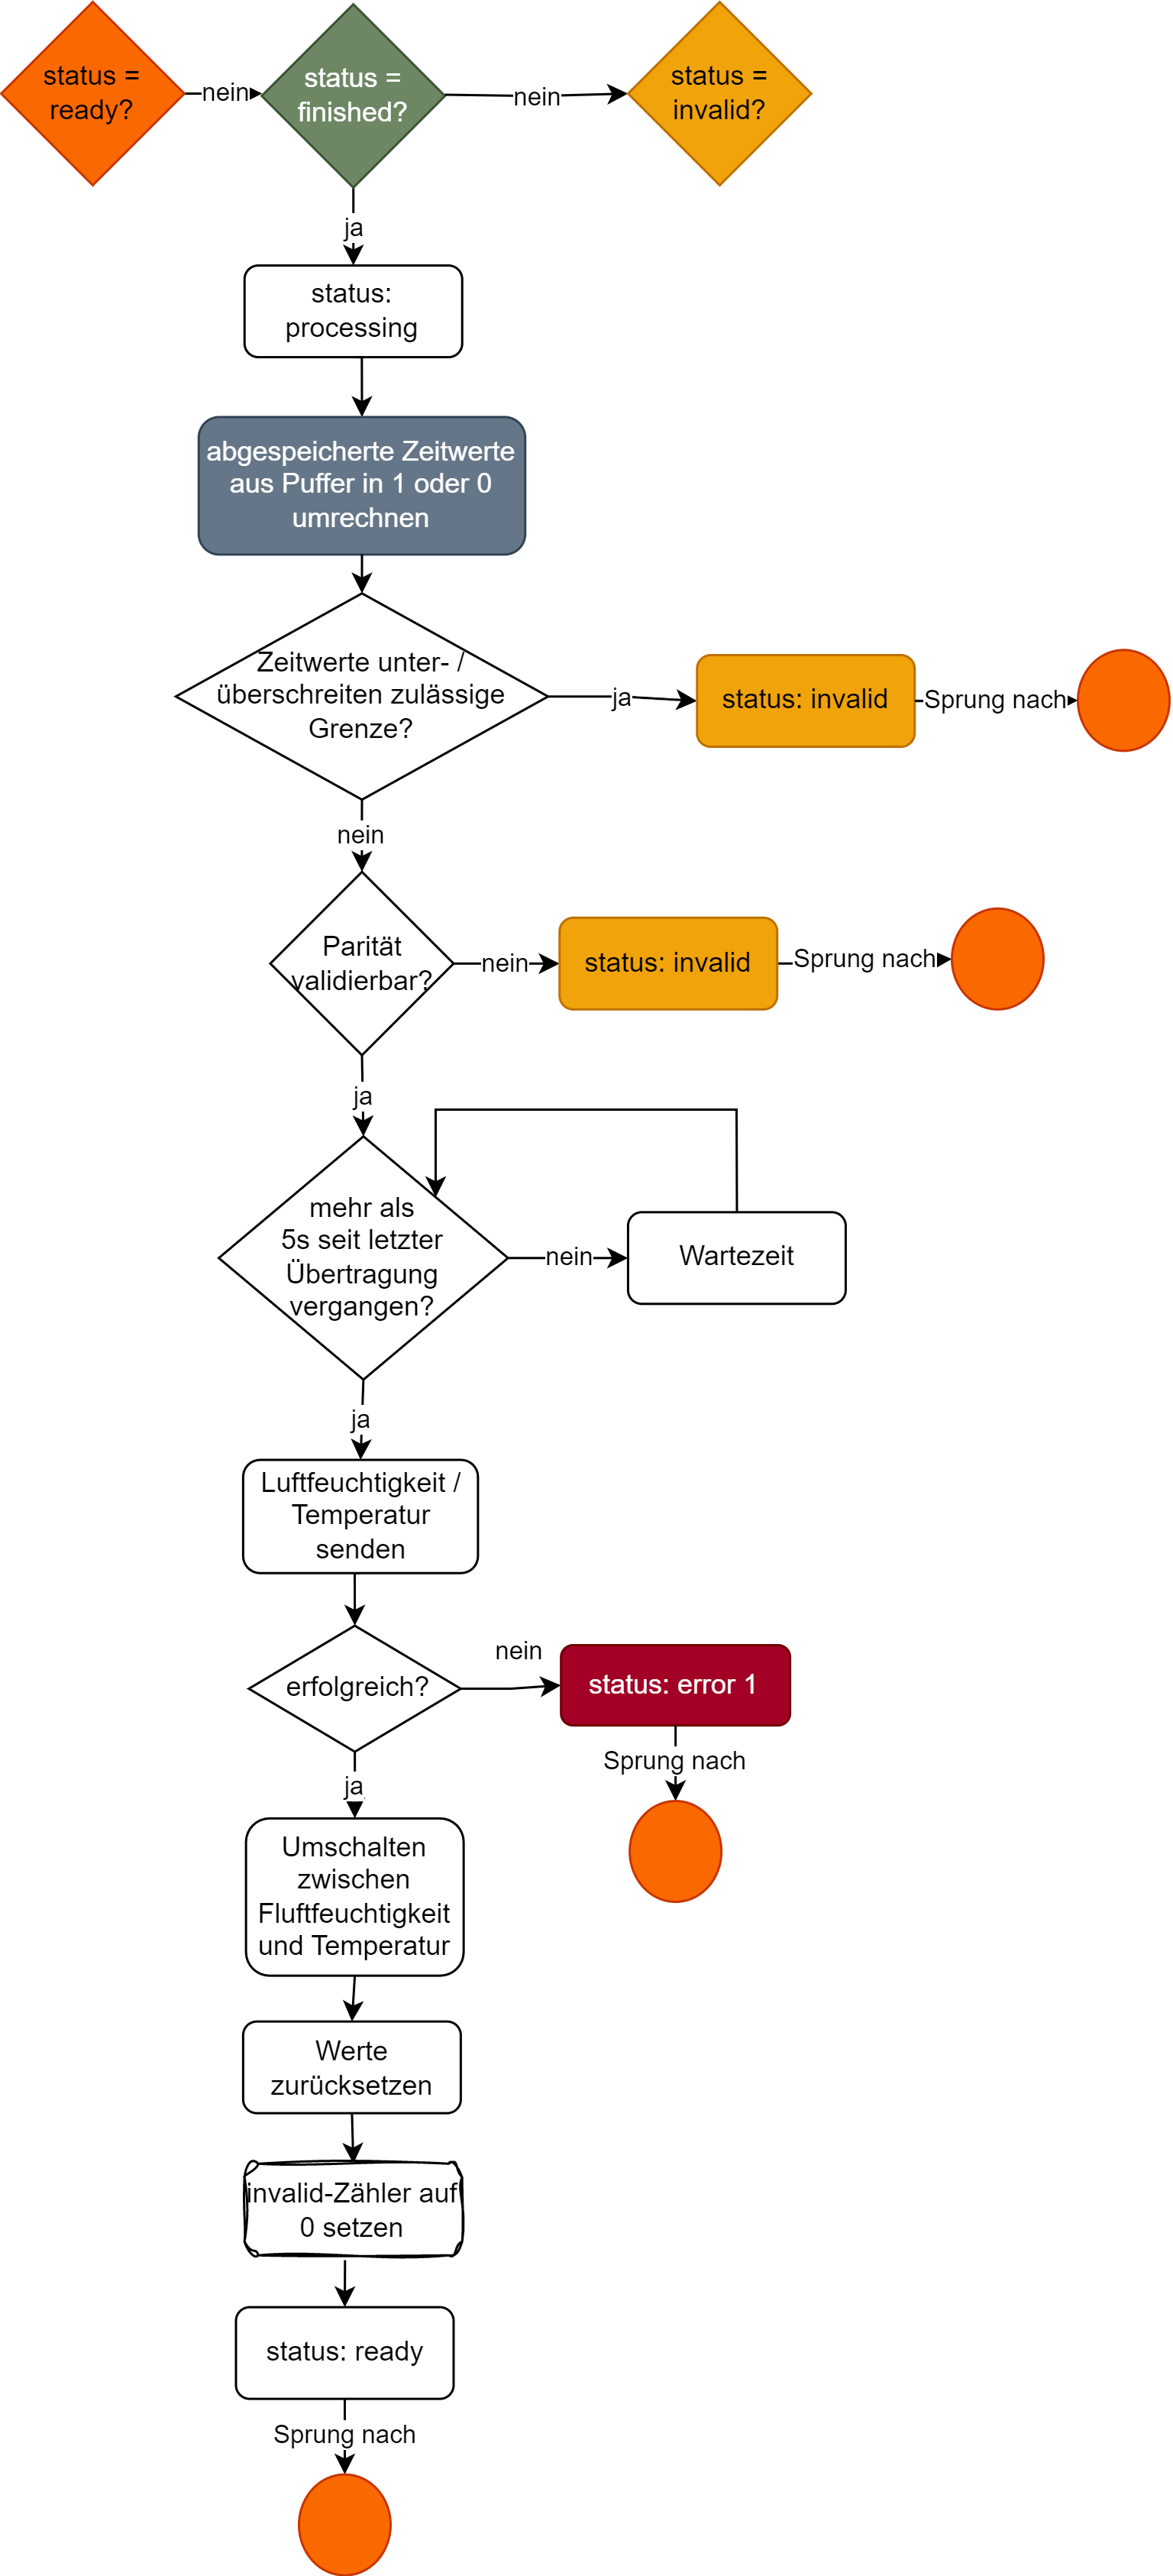
\includegraphics[height=0.9\textheight]{./Bilder-Tobit/flussdiagramm_finished.png}
    \caption{Flussdiagramm: fertiger Datensatz}
    \label{fig:flussdiagramm_finished}
\end{figure}

\begin{figure}[H]
    \centering
    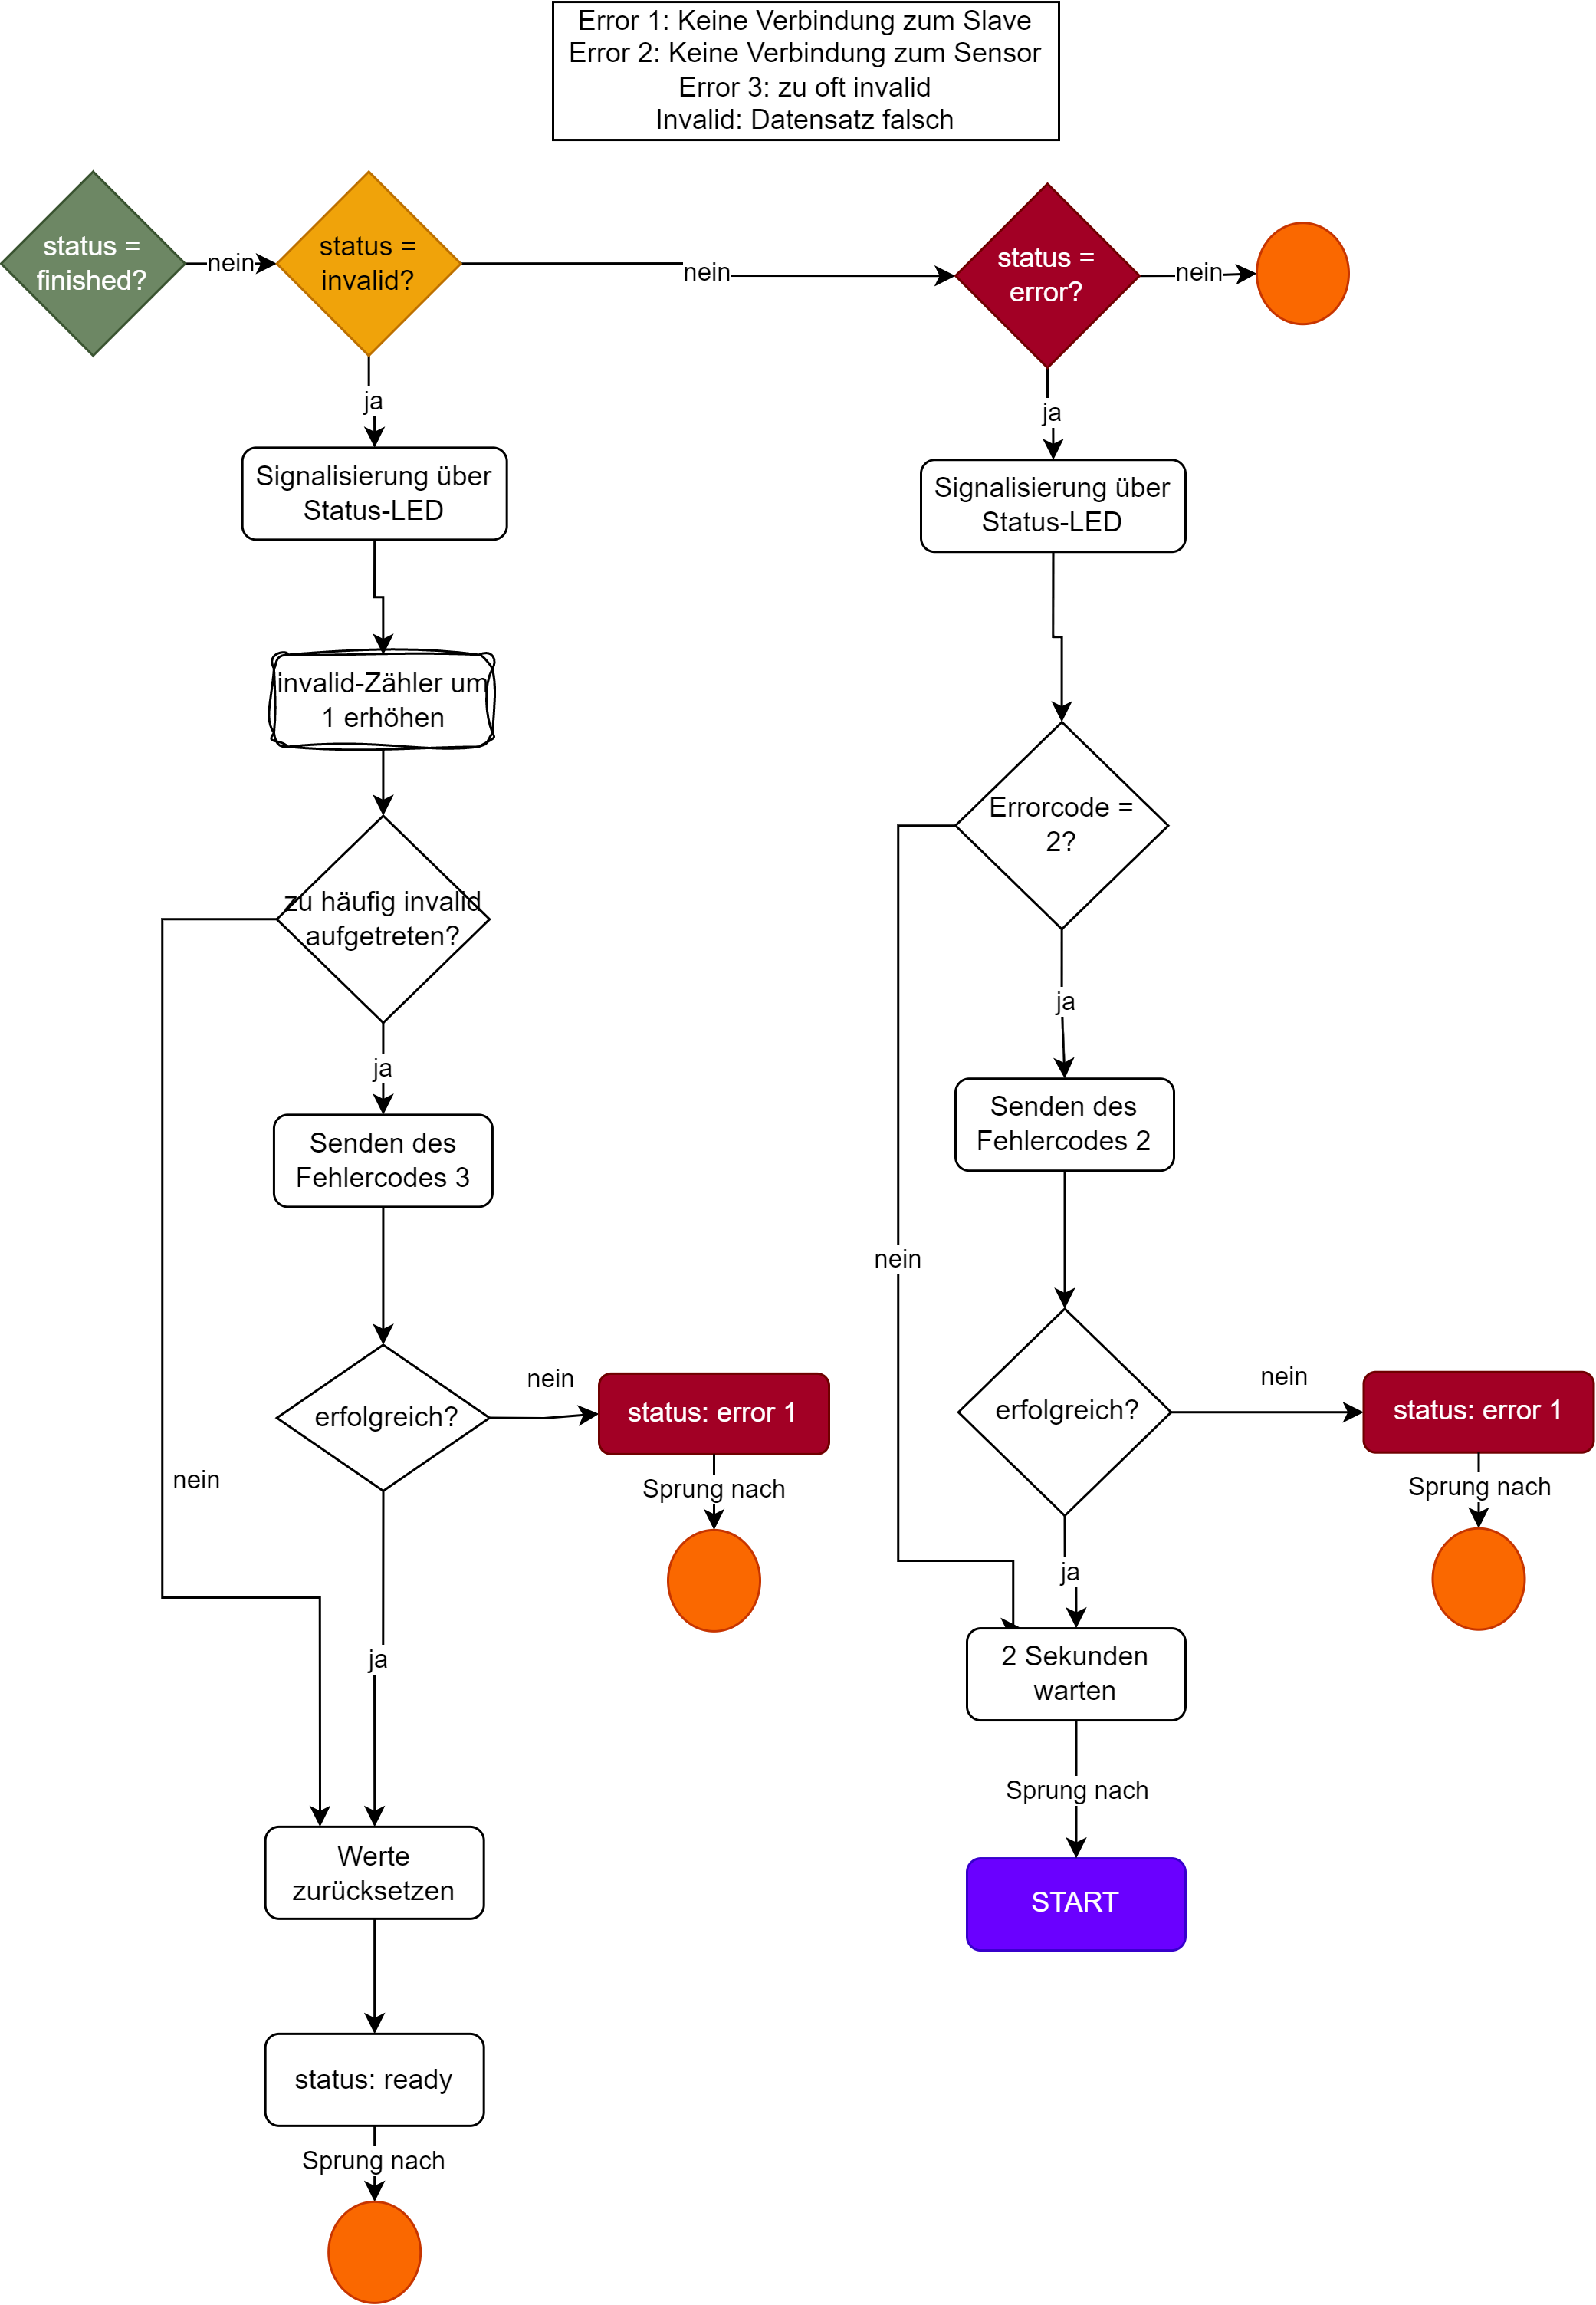
\includegraphics[height=0.9\textheight]{./Bilder-Tobit/flussdiagramm_invalid_error.png}
    \caption{Flussdiagramm: Fehlerbehandungen}
    \label{fig:flussdiagramm_invalid_error}
\end{figure}

\begin{figure}[H]
    \centering
    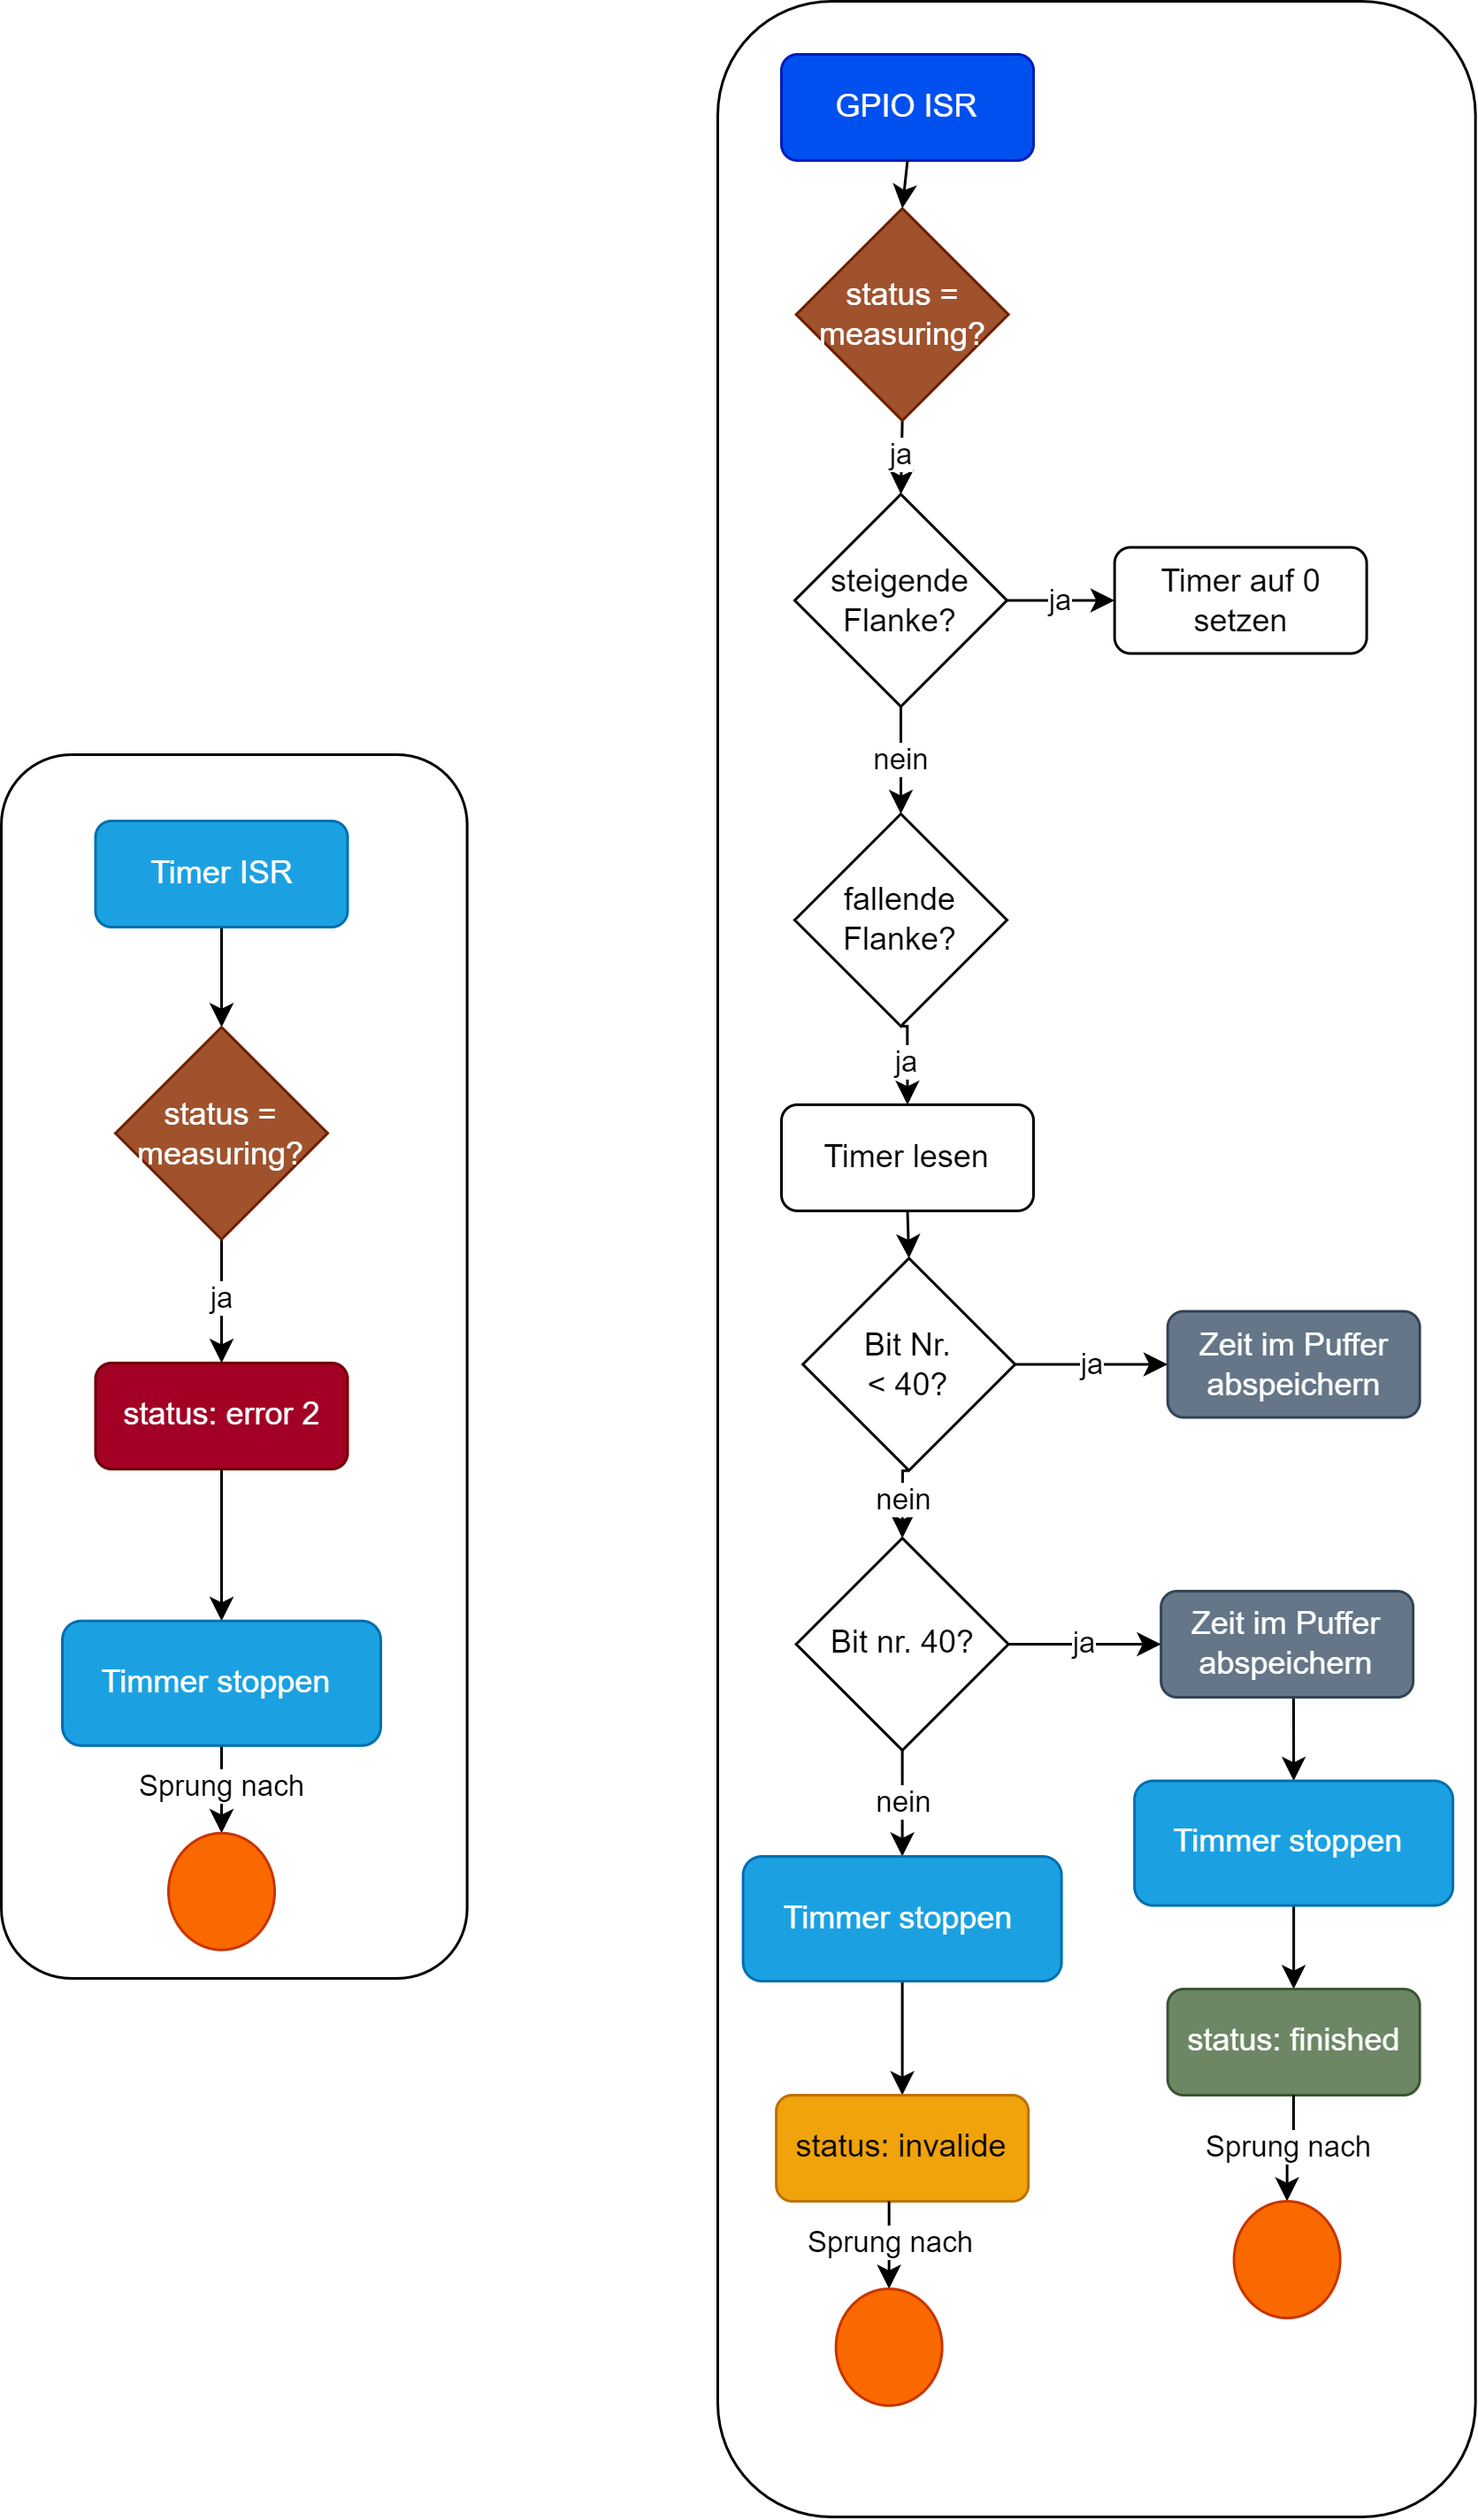
\includegraphics[height=0.9\textheight]{./Bilder-Tobit/flussdiagramm_ISR.png}
    \caption{Flussdiagramm: Interrupt-Serive-Routinen des Timers und des GPIOs}
    \label{fig:flussdiagramm_ISR}
\end{figure}

\newpage

Auf Grundlage dieses Flussdiagramms und der vorangegangenen Tests, konnte mit dem eigentlichen Coden begonnen werden.\\
Zunächst wurde ein neues Projekt mit allen benötigten Komponenten (Timer, I²C und GPIO mit Interruptfunktion) angelegt.
Zusätzlich wurden ein paar Kleinigkeiten bezüglich des Test-Projektes umgeändert.
\footnote{Beispielsweie wurde am Ende die Wartezeit zwischen senden des Startsignals und dem Freigeben der Leitung von 18ms auf 10ms reduziert.}

Der eigentliche Coding-Prozess soll an dieser Stelle eher unerwähnt bleiben,
da das Flussdiagramm zu großen teilen eins zu eins in C-Code übertragen werden konnte.
Auch die dabei aufgetretenen Fehler waren zunächst eher belanglos.\\

Allerding hier nun noch ein paar Elemente, die dennoch Erwähnung finden sollten.\\

1. Die Datensätze, welche vom Sensor gelesen werden bestehen aus 5 Bytes,
die ersten zwei entsprechnen der Luftfeuchtigkeit, die zweiten Bytes für die Temperatur und das letzte Byte ist die Parität.
Da nun die Luftfeuchtigkeit und die Temperatur zwei Bytes umfassen bietet sich der Datentyp \texttt{uint16\_t} an.
Zur Validierung muss allerdings die Summe der einzelnen Bytes das Paritätsbyte ergeben.\\
Die Lösungsstrategie, welche hier zum Einsatz kommt, ist ein \texttt{union}.\\
Ein union ermöglicht das Überlagern von Datentypen auf dem selben Speicher.
Übertragen auf dieses Problem, werden zwei \texttt{uint8\_t} Elemente auf dem selben Speicher,
wie ein \texttt{uint16\_t} gespeichert (siehe \cref{code:data_t}).
In \cref{code:union} ist die Umsetzung dokumentiert.\\
Mit \verb|.Uint16_t_1x| wird die Variable als \texttt{uint16\_t} interpretiert und
mit \verb|.Uint8_t_2x.firstByte| bzw. \verb|.Uint8_t_2x.secondByte| als zwei einzelne Bytes.

\begin{lstlisting}[language=C, label={code:data_t}, caption={Der \texttt{data\_t} Datentyp}]
struct halfData {
    uint8_t firstByte;
    uint8_t secondByte;
};

//used to interpret one uint16_t as two uint8_t
typedef union {
    uint16_t Uint16_t_1x;
    struct halfData Uint8_t_2x;
} data_t;
\end{lstlisting}

\begin{lstlisting}[language=C, label={code:union}, caption={Nutzung des \texttt{data\_t} Datentyps}]
dataset[humidity].Uint16_t_1x = dataset[humidity].Uint16_t_1x | 1 << (17 - element);
//...
sum = dataset[humidity].Uint8_t_2x.firstByte;
sum += dataset[humidity].Uint8_t_2x.secondByte;
sum += dataset[temperature].Uint8_t_2x.firstByte;
sum += dataset[temperature].Uint8_t_2x.secondByte;
if (parity != sum) {
    currentState = invalid;
    return;
}
\end{lstlisting}


2. Ein anderer Punkt stellt das Blockieren des \textit{measuring} Zustands dar.
Laut Datenblatt darf der Sensor maximal alle 2 Sekunden ausgelesen werden, da sonst die Daten unbrauchbar sind.\\
Hierfür wurde eine Sperre eingebaut, welche das Senden des Startsignals verhindert (siehe \cref{code:blockMeasurement}).
Die Sperre basiert auf dem System-Tick und einem Zeitstempel \Verb|tick_blockMeasurement|, der den Zeitpunkte der letzten Messung darstellt.\\
Im \cref{code:blockMeasurement} wird zunächst \Verb|HAL_GetTick()| von \Verb|tick_blockMeasurement| abgezogen.
Ist die letzte Messung älter als 2 Sekunden, ist die Differenz größer als 2000 und es kann eine neue Messung durchgeführt werden.\\
Läuft das System allerdings sehr lange (etwa 50 Tage), kommt es zu einem Überlauf der \textit{systick}-Variable.
\footnote{Die Systick Variable besteht aus 32 Bit.}
In diesem Fall würde \Verb|HAL_GetTick() - tick_blockMeasurement| nicht mehr die korrekte vergangene Zeit angeben,
denn die Differenz würde negativ werden.
Auf Grund des zyklischen Verhaltens, kann allerdings die negative Differenz in eine äquivalente positive Differenz umgerechnet werden (siehe \cref{fig:zyclus}).
Diese äquivalente Zahl wird dann überprüft, ob sie größer als 2000 ist.\\

\begin{figure}[H]
    \centering
    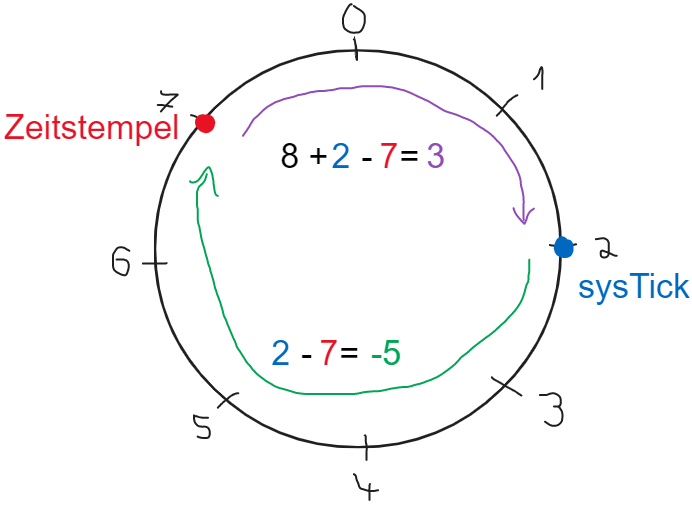
\includegraphics[width=0.5\textwidth]{./Bilder-Tobit/zyclus.png}
    \caption{Zyclus beim Überlauf}
    {\small Der Kreis enspricht dem Typ uint8, die -5 ist equivalent zur 3}
    \label{fig:zyclus}
\end{figure}

Der Initialwert von \Verb|tick_blockMeasurement| ist, anders als wie evtl. angenommen nicht 0,
sonst würde das System, bei der ersten Messung, 2 Sekunden warten.
Um dies zu verhindert wird das zyklische Verhalten ausgenutzt;
\Verb|tick_blockMeasurement| wird dabei mit  ``höchstmögliche 32-Bit Zahl minus 2000 Millisekunden'' initialisiert.
Dadurch ist die Differenz vom Start an, >=2000.
Samot kann die Messung ohne Blockierung starten.

\begin{lstlisting}[language=C, label={code:blockMeasurement}, caption={Blockieren des Startsignals}]
int64_t difference = HAL_GetTick() - tick_blockMeasurement;
//check for a systick overflow:
if (difference < 0) {
    difference = uint32NumValues + difference;
}
if (difference >= 2000) {
    //if more than 2 seconds have passed
    tick_blockMeasurement = HAL_GetTick();
    statusReady();
}
\end{lstlisting}

Damit ist die Bearbeitung der Sensor-Seite abgeschlossen.

Das System wurde anschließend erneut mit dem Arduino getestet
\footnote{Hier liegt die Software: \url{https://gitlab.rz.htw-berlin.de/s0582020/ce31-embd-gruppe-6-tz-kh/-/tree/main/Tobit/arduino_slave}}.
Dabei konne allerdings nicht der \textit{invalid} Zustand getestet werden.

Das Verbinden beider Systeme (Sensor-Seite und Darstellungs-Seite) sollte,
Aufgrund der definierten Schnittstellen zwischen beiden Nucleos,
reibungslos verlaufen.

\newpage
\subsection{4-stellige 7-Segment-Anzeige (Kevin Hübner)}
\label{sec:7-seg-anzeige}

\subsubsection{Grundlagen der 7-Segment-Anzeige}

Um die gemessenen Daten des Temperatur- und Luftfeuchtigkeitssensors anzeigen zu können wird eine 4-Stellige-7-Segment-Anzeige genutzt.
Vor der Implementierung wurde zuerst das Datenblatt
\footnote{\url{http://www.datasheet-pdf.com/PDF/TM1637-Datasheet-TitanMicro-788613}}
studiert.
Zudem hilft ein Github-Projekt\footnote{\url{https://github.com/UsefulElectronics/stm32-tm1637-library/}} bei der Implementierung,
dieses stellt wichtige Funktionen bereit, die unabdingbar funktionieren müssen.\\

Die 7-Segment-Anzeige bietet im Allgemeinen nur 4 Pins, welche mit dem Nucleo-Board oder anderen Boards verbunden werden.
Dabei gibt es einen Pin der mit GND verbunden wird und einen zweiten Pin der mit der Spannungsversorgung von 3.3 V des Nucleo-Boards verbunden wird.
Die anderen beiden Pins sind für die Datenübertragung (DIO-Pin) und den Clock-Input (CLK-Pin) zuständig.
Dafür werden am Nucleo-Board zwei GPIO-Pins im Output-Mode benötigt.
Auf Basis dieser Einstellungen wurde das Grundgerüst
\footnote{\url{https://gitlab.rz.htw-berlin.de/s0582020/ce31-embd-gruppe-6-tz-kh/-/commit/58021275a10379d7487f0d2c0f1618022f65e426}}
erstellt.\\

Im Datenblatt findet sich folgende Abbildung \cref{data-transfer}:

\vspace{1cm}
\begin{figure}[h]
    \begin{center}
        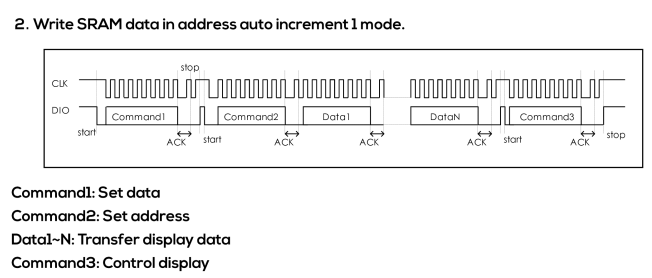
\includegraphics[width=\textwidth]{Bilder/Data-transfer.png}
        \caption{Datenübertragung bei der 7-Segment-Anzeige}
        \label{data-transfer}
    \end{center}
\end{figure}

Darinen ist ersichtlich, wie die Anzeige angesprochen wird.
Wichtige Information die hier mitgenommen werden können sind die Commands, die Start-Befehle, der Stop-Befehl und ACK.
Die Commands werden benötigt um das Displayregister zu beschreiben.\\

\newpage
Der Beispielablauf um etwas auf dem Display anzeigen zu lassen wäre also, laut Abbildung, wie folgt:\\
Schritt 1: Start-Befehl (Zum starten der Datenübertragung auf den Chip der Anzeige)\\
Schritt 2: Command 1 (Zum Festlegen ob gelesen oder geschrieben werden soll)\\
Schritt 3: Command 2 (Zum Festlegen der Adresse)\\
Schritt 4: Datensatz 1 (Zum Festlegen der aktiven Segmente an der ersten Stelle)\\
Schritt 5: Datensatz 2 (Zum Festlegen der aktiven Segmente an der zweiten Stelle)\\
Schritt 6: Datensatz 3 (Zum Festlegen der aktiven Segmente an der dritten Stelle)\\
Schritt 7: Datensatz 4 (Zum Festlegen der aktiven Segmente an der vierten Stelle)\\
Schritt 8: Command 3 (Zum Festlegen ob das Display an oder ausgeschaltet sein soll)\\
Schritt 9: Stop-Befehl (Zum stoppen der Datenübertragung)\\

Diese Schritte können sehr leicht runtergebrochen werden,
da fast alle benötigten Informationen im Datenblatt in der gleichen Reihenfolge zu finden sind.\\
Das Erste was einem Auffällt ist, dass jeder Command bzw. jeder Data-Befehl mit einem ACK endet.
Das heißt es wird auf eine Rückmeldung vom Micokontroller der 7-Segment-Anzeige gewartet und ist die einzige Input-Aktion,
welche beachtet werden muss.
Die Befehle für den Start bzw. Stop sind abhängig von der CLK/DIO-Flanke
und diese müssen in exakter Reihenfolge auf \textit{High} bzw. \textit{Low} geschaltet werden.\\
Für die Commands gibt es immer einen Start-Befehl, aber nur für den ersten Command gibt es einen Stop-Befehl,
jedoch kommt nach dem dritten Command ebenfalls ein Stop-Befehl um die Datenübertragung abzuschließen.
Die Datensätze sind unabhängig voneinander und beschreiben das Register der 7-Segment-Anzeige mit den Werten,
welche an der jeweiligen Stelle dargestellt werden soll.
Jede Stelle der Anzeige wird über ein 8-Bit (1 Byte) langes Register geschrieben.
Dabei ist zu beachten, dass die Binäre-Darstellung einer Zahl nicht gleich der Darstellung auf der Anzeige entspricht.
Jedes einzelne Segment entspricht einem Bit aus den 8-Bit des Registers d.h. um beispielsweise eine 1 auf der Anzeige darzustellen,
müssen zwei Bit im Register auf 1 gesetzt werden, das Segment \textit{b} sowie das Segment \textit{c} (siehe \cref{7sa}).

\vspace{1cm}
\begin{figure}[h]
    \begin{center}
        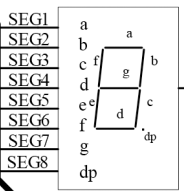
\includegraphics[scale=0.8]{Bilder/7-Segment-Display.png}
        \caption{7-Segment-Anzeige}
        \label{7sa}
    \end{center}
\end{figure}


\newpage

Jeder Command und jede 7-Segment-Stelle wird über 9 CLKs abgearbeitet (8 für die Daten und 1 für den ACK).
Insgesamt sind das bei den 4 Stellen der 7-Segment-Anzeige mit den 3 Commands, 7 dieser 9 CLK-Cyclen.



\subsubsection{Erste Inbetriebname der 7-Segment-Anzeige}

Die Pins, welche benötigt werden um die 7-Segment-Anzeige in Betrieb zu nehmen (DIO-Pin und CLK-Pin),
werden über die Software STM32 CubeMX (Pins PA6 | A5 und PA7 | A6 bei diesem Nucleo-Board) auf Output gestellt.
Beim Debuggen kann man noch den Pin PB3 des Nucleo-Boards als GPIO-Output setzen.
Der Pin kann dann genutzt werden, um eine Led zu steuern und dient als debug-Hilfe.\\

Da später Sensordaten von dem ersten Nucleo über I²C empfangen werden, wird zusätzlich I²C aktiviert.
Wichtig dabei ist noch die Aktivierung des I2C-Interrupthandlers und das Setzen der Slave-Adresse (hier 0x20) damit wir von einem Board,
welches als Master agiert, die Daten empfangen können.\\

Als Grundstein der Implementierung wird die Funktion \texttt{HAL\_GPIO\_WritePin} benötigt.
Mit dieser können die Pins, welche die Pegel für den CLK-Pin und DIO-Pin der Anzeige definieren,
auf \textit{High} bzw. \textit{Low} gestellt werden.
Durch das Ändern der Pegel wird dem Microkontroller der 7-Segment-Anzeige alle nötigen Informationen mitgeteilt.
Die Informationen liegen dabei als Bits, je nach Pegelzustand 0 oder 1, vor und werden an die Anzeige übergeben.
Es muss dabei beachtet werden, zu welchem Zeitpunkt ein bestimmter Wert an die Anzeige geschickt wird.\\

Als ersten Schritt wurde der Start- bzw. Stop-Befehl implementiert.
Über die vorher erwähnte Funktion \texttt{HAL\_GPIO\_WritePin} lassen sich beide Befehle leicht implementieren.
Es muss nur darauf geachtet werden, dass der richtige Pin zur richtigen Zeit \textit{Low} bzw. \textit{High} gesetzt wird.
Für den Start-Befehl wird die CLK auf \textit{High} gesetzt und während die CLK in diesem Zustand ist,
wird der DIO-Pin von \textit{High} auf \textit{Low} gesetzt (siehe Abbildung \ref{start}).
Für den Stop-Befehl wird der CLK-Pin ebenfalls auf \textit{High} gesetzt,
jedoch wird diesmal der DIO-Pin von \textit{Low} auf \textit{High} gezogen (siehe Abbildung \ref{stop}).\\
Mithilfe eines Logic Analyzers wurde anschließend getestet, ob die Flanken der Stop- bzw. Start-Funktion zum richtigen Zeitpunkt eintreffen.\\

\vspace{0.7cm}
\begin{figure}[h]
    \begin{center}
        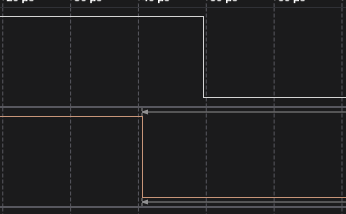
\includegraphics[width=0.6\textwidth]{Bilder/start_cmd.png}
        \caption{Start-Befehl über die Flanken des Nucleo-Boards}
        {\small oben: CLK, unten: DIO}
        \label{start}
    \end{center}
\end{figure}
\begin{figure}
    \begin{center}
        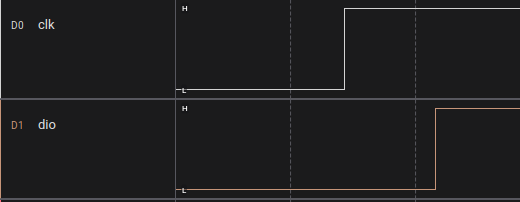
\includegraphics[width=0.6\textwidth]{Bilder/stop_command.png}
        \caption{Stop-Befehl über die Flanken des Nucleo-Boards}
        \label{stop}
    \end{center}
\end{figure}

\newpage

Ebenfalls wichtig für das Projekt ist der Acknowledgment-Check (ACK-Check).
Nach jedem abgearbeiteten 9-CLK-Cycle wird eine Antwort (ACK) erwartet.
Da jedoch beide GPIO-Pins auf Output gestellt sind, kann keiner der beiden Pins ein ACK entgegennehmen.
Hier ist es wichtig den CLK-Pin kurzzeitig auf Input zu setzen und auf diesen ACK zu warten.
Um einen Pin als Input zu deklarieren, wird dieser per \texttt{GPIO\_InitStruct.Mode} auf \texttt{GPIO\_MODE\_INPUT} gesetzt.
Für die ACK-Check-Funktion muss der Pin-Zustand geändert werden (Output -> Input -> Output wenn ACK erfolgt ist)
und es muss auf den ACK gewartet werden. Das wurde, für dieses Projekt,
in der Funktion \textit{display\_check\_acknowledge} (Abbildung \cref{ack}) realisiert.


\begin{lstlisting}[language=C, label={ack}, caption={Funktion zum Überprüfen des Acknowledgements}]
void display_check_acknowledge()
{
	change_pin_mode(input);
	display_clk_low();

	while(HAL_GPIO_ReadPin(CLK_GPIO_Port, CLK_Pin))
	{
		HAL_GPIO_WritePin(led_GPIO_Port, led_Pin,SET);
		
	}
	HAL_GPIO_WritePin(led_GPIO_Port, led_Pin,RESET);
	change_pin_mode(output);
}
\end{lstlisting}




Im Hauptteil des Programms fehlt nur noch eine Methode, um mithilfe von CLK und DIO die Anzeige so zu manipulieren,
sodas die gewünschten Zeichen angezeigt werden.\\

Der zu übertragenden Command bzw. die zu übertragenden Daten einer 7-Segment-Stelle liegen dabei in Arrays vor.
Das Ziel ist es nun mit jedem CLK-Schlag (\textit{Low}->\textit{High}->\textit{Low}) 
ein Bit über den DIO-Pin an die Anzeige zu senden (Beispiel in \cref{clk}).
Das jeweilige Bit wird über Bitshifting aus dem entsprechenden Array herausgefiltert.\\
Jeder Command bzw. jeder Datensatz wird über 9-CLKs in einer Periode umgesetzt.

\vspace{0.5cm}
\begin{figure}[h]
    \begin{center}
        \includegraphics[width=0.7\textwidth]{Bilder/daten_übertragung.png}
        \caption{CLK-Cyklus}
        {\small oben: CLK, unten: DIO}
        \label{clk}
    \end{center}
\end{figure}

\newpage

Desweiteren ist zu beachten, dass jeder Command bzw. Datensatz mit einem Start-Befehl beginnt, jedoch nicht mit einem Stop-Befehl aufhört.
Somit lohnt es sich zwei Funktionen zu schreiben, eine um die Commands ab zu arbeiten und eine andere um die Datensätze abzuarbeiten.

Für den Command 1 wird 0x40 (binär 0b0100 0000) zur Anzeige gesendet.
Dieser Wert legt fest, dass in folgende Register geschieben wird, 
das die Adresse automatisch Inkrementiert wird und es aktiviert den normal Mode.\\
In Command 2 wird die Startadresse gewählt, welche beschrieben werden soll.
Laut Datenblatt ist dies die Adresse C0H, mit dem 8-Bit Wert 0xC0 oder in binär 0b11000000.\\
Danach folgen die Datensätze, mit denen die 7-Segment-Stellen beschrieben werden.\\
Über Command 3 lässt sich die Anzeige an und ausschalten, aber auch die Helligkeit manipulieren.
In diesem Projekt ist die Helligkeit irrelevant.
Die Anzeige lässt sich mit 0x80 (0b10000000) ausschalten und mit 0x88 (0b10001000) einschalten.\\


In \cref{display_on} wurden die drei Commands sowie vier mal der Datensatz 0x3F (0x3F etspricht einer 0) an das Display übertragen 
und mit einem Logic Analyzer untersucht.

\vspace{1cm}
\begin{figure}[h]
    \begin{center}
        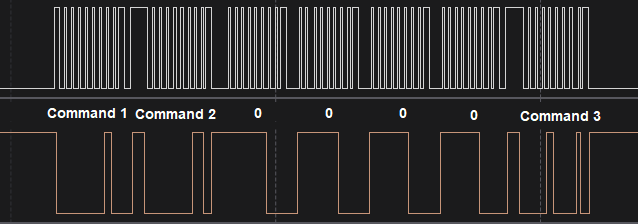
\includegraphics[width=0.7\textwidth]{Bilder/display_on_2.png}
        \caption{Logic Analyzer für das anschalten des Displays}
        {\small oben: CLK, unten: DIO, Beispielübertragen stellt vier Nullen dar.}
        \label{display_on}
    \end{center}
\end{figure}

\newpage

Als Beispiel\footnote{\url{https://gitlab.rz.htw-berlin.de/s0582020/ce31-embd-gruppe-6-tz-kh/-/commit/7f20b1f06ab9d345955305177ffee06c94a51b81}}
wurde auf der Anzeige 0000 ausgegeben (siehe \cref{display}).
Dabei blieb die Anzeige periodisch für 5 Sekunden (über die HAL\_Delay-Funktion) eingeschaltet 
und für 2.5 Sekunden im ausgeschalteten Zustand.

\vspace{1cm}
\begin{figure}[h]
    \begin{center}
        \includegraphics[width=0.7\textwidth]{Bilder/display_p.png}
        \caption{Angeschaltetes Display}
        \label{display}
    \end{center}
\end{figure}


\subsubsection{I2C Anpassungen}
Nun ist die Implementierung der Anzeige so gut wie fertig:
Daten können manuell auf das Display schreiben werden und das Display kann An bzw. Ausgeschalten werden.
Da jedoch Daten von einem weiteren Nucleo, welche mit einem Sensor verbunden ist,
empfangen werden, ist es notwendig die I2C-Kommunikation zwsichen den Boards zutesten.
Aus diesem Grund wurde ein neues Test-Projekt erstellt.\\
Als Testen wird hier zunächst ein Arduino genutzt, welcher als Master Daten sendet.\\

Für dieses Testprojekt wird eine LED, sowie die I2C-Kommunikation aktiviert.
Da dieses Nucleo-Board, welches die Darstellung der Luft- und Temperaturwerte übernimmt, 
als Slave arbeitet wird in den I2C-Einstellung noch die Slaveadresse 0x20 eingetragen.
\footnote{Für die Seite des I2C-Slaves wurde sich hieran orientiert: \url{https://community.st.com/s/article/how-to-create-an-i2c-slave-device-using-the-stm32cube-library}\\
und hier: \url{https://www.st.com/resource/en/user_manual/dm00173145-description-of-stm32l4l4-hal-and-lowlayer-drivers-stmicroelectronics.pdf}}
Diese Adresse wird später vom Master adressiert.
Desweiteren wird für I2C der Interruptmodus eingeschaltet.\\

Um allerding zwischen den Boards kommunizieren zu können, werden noch zwei PullUp-Widerstände für die Daten- und Clockverbindung hinzugefügt.\\

Mit den vorgenommenen Einstellungen und der LED kann überprüft werden, ob die Kommunikation zwischen beiden Boards funktioniert.\\

I2C kann in drei verschiedenen Modi genutzt werden: per Polling, per Interrupt und per DMA.
Im ersten Test wird Polling genutzt, da es sich um die einfachere Methode handelt.
Der Master sendet dabei den Wert 0x40FF und der Slave empfängt diesen über die Funktion \texttt{HAL\_I2C\_Slave\_Receive (Polling)}.
Bei Polling wartet der Slave so lange auf eine Nachricht, bis ein Timeout überschritten wurde.

Der Versuch mit Polling
\footnote{\url{https://gitlab.rz.htw-berlin.de/s0582020/ce31-embd-gruppe-6-tz-kh/-/commit/f0cb88f215dd76c01cb24b5267ed8661962d2888}}
sieht dann wie folgt aus: \cref{i2c}.

\begin{figure}[h]
    \begin{center}
        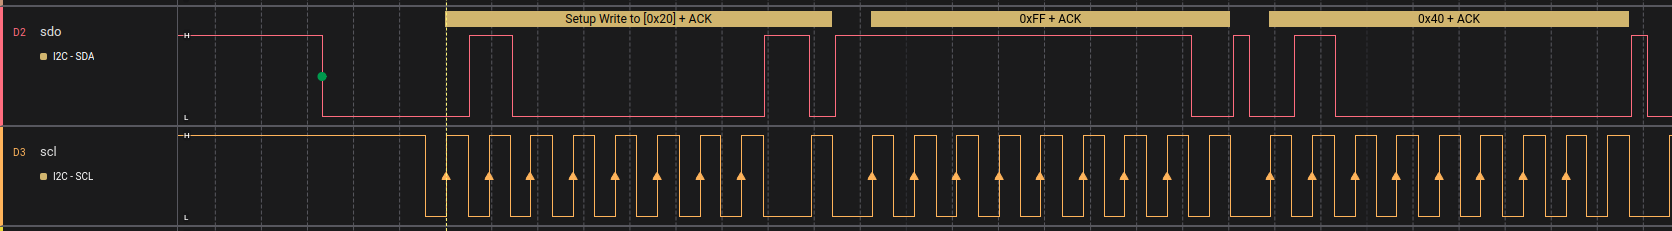
\includegraphics[width=1.1\textwidth]{Bilder/i2c_pollling.png}
        \caption{I2C Ergebnis der Kommunikation über Polling (erster Datensatz)}
        \label{i2c}
    \end{center}
\end{figure}

Im zweiten Test wird der Interruptmodus von I2C ausgetestet.\\
\footnote{\url{https://gitlab.rz.htw-berlin.de/s0582020/ce31-embd-gruppe-6-tz-kh/-/commit/8dc36db574aa064f33940e40cb78256e63d41787}}
Dieser wird über die Funktion \\\texttt{HAL\_I2C\_Slave\_Receive\_IT (Interrupt)} gestartet.
Desweiteren wird eine Callback-Funktion \texttt{HAL\_I2C\_SlaveRxCpltCallback} benötigt.
Diese wird automatisch vom System aufgerufen, sobald der Slave einen vollständigen Datensatz erhalten hat.\\

Für diesen Test sendet der Master zunächst beliebige Werte mit der Länge von zwei Bytes.\\
In der Callback-Funktion wird die LED umgeschaltet, d.h. zwischen angeschaltet und ausgeschaltet gewechselt.
Damit lässt sich visuell feststellen, ob der Aufruf der Callback-Funktion gelungen ist.
Entspricht der empfange Wert dem Wert 0xCAFE, 
so sendet der Slave mit der Funktion \texttt{HAL\_I2C\_Slave\_Transmit} die Antwort 0x55 zum Master. (siehe \cref{i2c-interrupt})

\begin{figure}[h]
    \begin{center}
        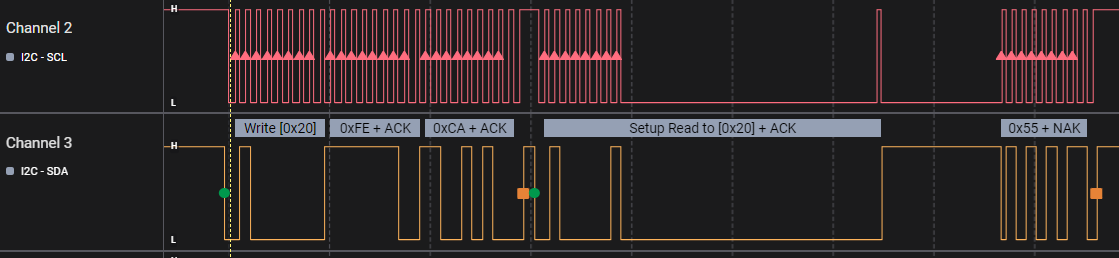
\includegraphics[width=\textwidth]{Bilder/i2c_interrupt.PNG}
        \caption{I2C Ergebnis der Kommunikation über Interrupt}
        \label{i2c-interrupt}
    \end{center}
\end{figure}

Somit ist die Kommunikation mit I2C für das Testprojekt
\footnote{\url{https://gitlab.rz.htw-berlin.de/s0582020/ce31-embd-gruppe-6-tz-kh/-/commit/8dc36db574aa064f33940e40cb78256e63d41787}}
geglückt und für das eigentliche Projekt nun beide Teile: Display und I2C zusammengeführt.


\subsubsection{Zusammenführung von Display und I2C}
In diesem Schritt wird die Darstellung auf dem Displays mit der Kommunikation zum anderen Nucelo-Board zusammengeführt.\\

Dabei sind noch einige Dinge zu beachten:\\
Das erste Board, welches den Sensor ausliest, sendet abwechselnd Luftfeuchtigkeit und Temperatur.
Zur Unterscheidung, wird in dem vorletzten Bit kodiert, ob es sich um Luftfeuchtigkeit oder Temperatur handelt.
Luftfeuchtigkeit entspricht einer 0 und 1 ist Temperatur.
Über eine Bitmaske und Bitweisen UND wird die entsprechende Größe herausgefiltert.
auf dem Display wird die erste Stelle genutzt, um anzuzeigen, ob sich um eine Temperatur oder um Luftfeuchtigkeit handelt;
Für die Temperatur wird ein \textit{C} für Celsius dargestellt und für Luftfeuchtigkeit ein \textit{H} (Humidity).\\

Das erste Bit beschreibt, im Falle der Temperatur, der Vorzeichen.\\
Bit gesetzt bedeutet eine negative Temperatur und in der zweiten Stelle der Anzeige wird ein \textit{'-'} angezeigt,
sond ist die Stelle leer.\\

Die beiden letzten Stellen der Anzeige nehmen die gemessenen Werte ein.
Da nun alle vier Stellen belegt sind, wurde sich dazu entschieden, auf die Nachkommastellen zu verzichten.\\

Doch ohne Nachkommastellen müssen die Zahlen gerundet werden was zu einem weiteren Problem führt.
Die Daten aus 2 Byte enthalten in den ersten zwei Stelle (MSB und MSB-1) die Codierung,
welche entscheidet ob es sich um eine Temperatur oder eine Luftfeuchtigkeit handelt.
Diese wird über eine Bitmaske entfernt, damit die Daten als Wert interpretiert werden können.
Für die Anzeige ist es notwendig den Wert so vorzubereiten, dass die Zehner- und Einer-Stellen in jeweils 8 Bits binär vorliegen.
Das Stichwort dazu lautet BCD-Code.\\
Beispielsweie die Zahl 13 sieht binär, in 16 Bits, so aus: 0b0000000000001101.
Um die 13 auf der Anzeige darzustellen, muss die 13 in zwei verchiedene 8 Bits aufgeteilt werden.
Die 1 (Zehner) wird in 0b00000010 und die 3 (Einer) in 0b00000011 umgewandelt.
Der Algorithmus
\footnote{\url{https://en.wikipedia.org/wiki/Double_dabble}}
ist in der Double\_Dabble-Funktion in \cref{dd} implementiert.



\begin{lstlisting}[language=C, label={dd}, caption={Double Dabble Funktion}]
void double_dabble(uint8_t data) {
	union dd wandler;
	wandler.num = 0x00;

	wandler.raw.input_data = data;

	for (int i = 0; i < 7; i++) {
		wandler.num = wandler.num << 1;
		if (wandler.raw.zehner >= 5) {
			wandler.raw.zehner += 3;

		}
		if (wandler.raw.einer >= 5) {
			wandler.raw.einer += 3;

		}
	}
	wandler.num = wandler.num << 1;

	dd_data = wandler;
}

\end{lstlisting}



Ein Fehlerfall wird auf das Anzeige über ``ErrX'' dargestellt, wobei X den Fehlercode darstellt.
Im Datensatz des Masters wird Error über das setzen er obersten zwei Bits (MSB und MSB-1) kodiert.

Damit wäre alles notwendige implementiert.\\

Wie beim ersten Nucleo, basiert auch dieses System auf einer einfachen Zustandsmaschine.
Während des StartUps wartet der Slave darauf, dass der Master 0xCAFE sendet, wodurch der Slave in den Zustand \textit{active} versetzt wird.
Das ist der Schlüssel, in die Hauptschleife des Systems zu gelangen.
Einmal in die Hauptschleife gelangt, wartet das System nun ununterbrochen auf neue Datensätze, 
die dargestellt werden können.\\
Werden neue Datensätze empfangen, so wird der Status auf \textit{work} gesetzt und der Datensatz wird auf der Anzeige dargestellt.
Nach erfolgreichem aktuallisieren des Displays wird der Status auf \textit{no-work} geändert, um in den IDLE-Modus zurück zu kehren.\\

Bleiben für mehr als 10 Sekunden neue Datensätze aus, so wird ein Fehler auf dem Display angezeigt.

Und im Fall, dass es keine Verbindung zum Display gibt, blink die LED auf dem Board.

Das Projekt
\footnote{\url{https://gitlab.rz.htw-berlin.de/s0582020/ce31-embd-gruppe-6-tz-kh/-/commit/bbc1329171e7bb3871fb4049f9456aa00d5a023f}}
für die 4-Stellen-7-Segment-Anzeige ist damit fertig gestellt.

\subsection{Zusammenführung beider Systeme}
Nach Beendigung beider Implementierungen, konnten beide Systeme tatsächlich Problemlos verbunden werden (siehe \cref{fig:success}).

\begin{figure}[H]
    \begin{center}
        \includegraphics[width=\textwidth]{Bilder-Tobit/connection.jpg}
        \caption{Erfolgreiches Verbinden beider Nucleos}
        \label{fig:success}
    \end{center}
\end{figure}


\newpage

\section{Probleme}

Während der Tests der I2C-Kommunikation kam es zwischenzeitig zu Problemen:
1. Wurde der CLK-Pegel nach Polling-Timeouts vom Slave dauerhaft auf \textit{Low} gezogen (siehe \cref{fig:clk_low}).
Das Problem konnte durch die Einstellung \textit{Clock No Strech Mode} behoben werden.
Dabei war diese Einstellung im Reiter Connectivity auf Disable gestellt, jedoch muss diese auf Enable gestellt werden.\\

\begin{figure}[H]
    \begin{center}
        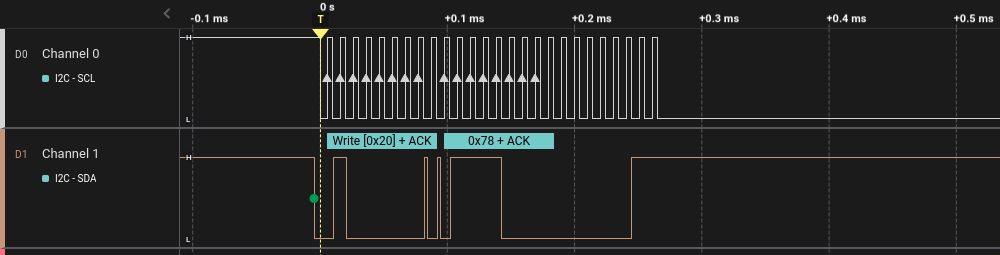
\includegraphics[width=\textwidth]{Bilder-Tobit/i2c-problem_clk-low_2.png}
        \caption{I2C Clock wird vom Slave auf \textit{Low} gezogen}
        \label{fig:clk_low}
    \end{center}
\end{figure}

2. Es wurde fälschlicher Weise während der Tests die Funktion \texttt{HAL\_I2C\_EnableListen\_IT} in den Code hinzugefügt,
allerdings trat damit eher das Gegenteil auf als wie der Name vermuten lässt.
Der Slave reagierte damit gar nicht mehr (siehe \cref{fig:no_response}).
Nach herausnehmen dieser Funktion lief das Verhalten die geplant.

\begin{figure}[H]
    \begin{center}
        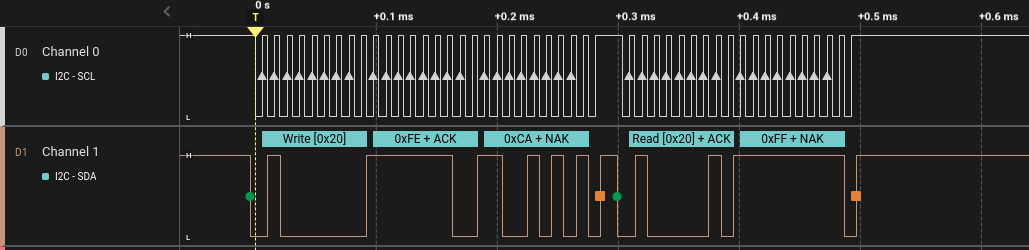
\includegraphics[width=\textwidth]{Bilder-Tobit/i2c-problem_no-slave-response.png}
        \caption{I2C Slave reagiert nicht}
        \label{fig:no_response}
    \end{center}
\end{figure}

\section{Fazit}
Das Projekt lief im Großen und Ganzen recht flüssig, auch wenn es ein paar größere Hürden zu überwinden galt.

Aufgrund von anderen zeitnahen Abgaben in anderen Modulen, war es notwendig das Projekt schnellstmöglich fertigzustellen,
dies ging leider auf Kosten der Dokumentationsqualität.

Als Weiterentwicklung könnten sämtliche \texttt{HAL\_Delay}-Funktionen ersetzt werden durch eine ökonomischere Methode;
so könnte sich der Mikrocontroller schlafen legen und über einen Timerinterrupt nach entsprechender Zeit wieder geweckt werden.

\end{document}